\lab{Introduction to Wavelets}{Introduction to Wavelets}
\objective{Wavelets are used to sparsely represent information.
This makes them useful in a variety of applications.
We explore both the one- and two-dimensional discrete wavelet transforms using various types of wavelets.
% HERE (above line): added hyphen after "one"
We then use a Python package called PyWavelets for further wavelet analysis including image cleaning and image compression.
}

\section*{Wavelet Functions}

\emph{Wavelets families} are sets of orthogonal functions (wavelets) designed to decompose nonperiodic, piecewise continuous functions.
These families have four types of wavelets: mother, daughter, father, and son functions.
Father and son wavelets contain information related to the general movement of the function, while mother and daughter wavelets contain information related to the details of the function.
The father and mother wavelets are the basis of a family of wavelets.
Son and daughter wavelets are just scaled translates of the father and mother wavelets, respectively.

\subsection*{Haar Wavelets}

The \emph{Haar Wavelet} family is one of the most widely used wavelet families in wavelet analysis.
This set includes the father, mother, son, and daughter wavelets defined below.
The Haar father (scaling) function is given by
\[
\varphi(x) =
 \begin{cases}
 1 & \text{if } 0 \leq x < 1 \\
 0 & \text{otherwise.}
 \end{cases}
\]
The Haar son wavelets are scaled and translated versions of the father wavelet:
\[
\varphi_{jk}(x)=\varphi(2^jx-k) =
 \begin{cases}
 1 & \text{if }\frac{k}{2^j} \leq x < \frac{k+1}{2^j} \\
 0 & \text{otherwise.}
 \end{cases}
\]
The Haar mother wavelet function is defined as
\[
\psi(x) =
 \begin{cases}
  1 & \text{if } 0 \leq x < \frac{1}{2} \\
  -1 & \text{if } \frac{1}{2} \leq x < 1 \\
  0 & \text{otherwise.}
 \end{cases}
\]
The Haar daughter wavelets are scaled and translated versions of the mother wavelet
\[
\psi_{jk}=\psi(2^jx-k)
\]
% It might be nice to plot this function and include the image in the lab.

\subsection*{Wavelet Decompositions}

Information (such as a mathematical function or signal) can be stored and analyzed by considering its \emph{wavelet decomposition}.
A \emph{wavelet decomposition} is a linear combination of wavelets.
For example, a mathematical function $f$ can be approximated as a combination of Haar son and daughter wavelets as follows:
\begin{align*}
f(x) = \sum_{k=-\infty}^{\infty} a_k\varphi_{m,k}(x) + \sum_{k=-\infty}^{\infty} b_{m,k}\psi_{m,k}(x) + \dots + \sum_{k=-\infty}^{\infty} b_{n,k}\psi_{n,k}(x)
\end{align*}
where $m<n$, and all but a finite number of the $a_k$ and $b_{j,k}$ terms are nonzero.
The $a_k$ terms are often referred to as \emph{approximation coefficients} while the $b_{j,k}$ terms are known as \emph{detail coefficients}.
The approximation coefficients typically capture the broader, more general features of a signal while the detail coefficients capture smaller details and noise.

A wavelet decomposition can be done with any family of wavelet functions.
Depending on the properties of the wavelet and the function (or signal) $f$, $f$ can be approximated to an arbitrary level of accuracy.
Each arbitrary wavelet family has a mother wavelet $\psi$ and a father wavelet $\varphi$ which are the basis of the family.
A countably infinite set of wavelet functions (daughter and son wavelets) can be generated using dilations and shifts of the first two functions where $m,k \in \mathbb{Z}$:
\begin{align*}
\psi_{m,k}(x) &= \psi(2^mx - k)\\
\varphi_{m,k}(x) &= \varphi(2^mx - k).
\end{align*}

\subsection*{The Discrete Wavelet Transform} % ===================================

The mapping from a function to a sequence of wavelet coefficients is called the \emph{discrete wavelet transform}.
The discrete wavelet transform is analogous to the discrete Fourier transform.
Now, instead of using trigonometric functions, different families of basis functions are used.


\begin{comment}
In the case of finitely-sampled signals and images, only finitely many wavelet coefficients are nonzero.
Depending on the application, we are often only interested in the coefficients corresponding to a subset of the basis functions.
Since a given family of wavelets forms an orthogonal set, we can compute the wavelet coefficients
by taking inner products (i.e. by integrating). This direct approach is not particularly efficient,
however. Just as there are fast algorithms for computing the Fourier transform (e.g. the FFT),
we can efficiently calculate wavelet coefficients using techniques from signal processing.
In particular, we will use an \emph{iterative filter bank} to compute the transform.
% mathematical derivation?
\end{comment}

In the case of finitely-sampled signals and images, there exists an efficient algorithm for computing the wavelet decomposition.
Commonly used wavelets have associated high-pass and low-pass filters which are derived from the wavelet and scaling functions, respectively.

When the low-pass filter is convolved with the sampled signal, low frequency (also known as approximation) information is extracted.
This is similar to turning up the bass on a speaker, which extracts the low frequencies of a sound wave.
This filter highlights the overall (slower-moving) pattern without paying too much attention to the high frequency details and extracts the approximation coefficients.%, which to the eye (or ear) may be unhelpful noise.

When the high-pass filter is convolved with the sampled signal, high frequency information (also known as detail) is extracted.
This is similar to turning up the treble on a speaker, which extracts the high frequencies of a sound wave.
This filter highlights the small changes found in the signal and extracts the detail coefficients.

The two primary operations of the algorithm are the discrete convolution and downsampling, denoted $*$ and $DS$, respectively.
First, a signal is convolved with both filters.
The convolutions fold the signal back on itself so the resulting array is the same size but half the information is duplicated, \emph{downsampling} is then required to eliminate the repeated information.
% Downsampling is the process of removing unimportant entries from an array.
In the context of this lab, a \emph{filter bank} is the combined process of convolving with a filter, and then downsampling.
The result will be an array of approximation coefficients $A$ and an array of detail coefficients $D$.
This process can be repeated on the new approximation to obtain another layer of approximation and detail coefficients.
See Figure \ref{fig:filter bank}.

A common lowpass filter is the averaging filter.
Given an array \textbf{x}, the averaging filter produces an array \textbf{y} where $y_n$ is the average of $x_n$ and $x_{n-1}$.
In other words, the averaging filter convolves an array with the array $L=\begin{bmatrix}\frac{1}{2} & \frac{1}{2}\end{bmatrix}$.
This filter preserves the main idea of the data.
The corresponding highpass filter is the distance filter.
Given an array \textbf{x}, the distance filter produces an array \textbf{y} where $y_n$ is the distance between $x_n$ and $x_{n-1}$ ($|x_n - x_{n-1}|$).
In other words, the difference filter convolves an array with the array $H=\begin{bmatrix}-\frac{1}{2}&\frac{1}{2}\end{bmatrix}$.
This filter preserves the details of the data.

For the Haar Wavelet, we will use the lowpass and highpass filters mentioned.
In order for this filters to have inverses, the filters must be normalized (for more on why this is, see Additional Materials).
The resulting lowpass and highpass filters for the Haar Wavelets are the following:
\begin{comment}
\begin{align*}
H &= \sqrt{2}\begin{bmatrix}\frac{1}{2} & \frac{1}{2}\\-\frac{1}{2} & \frac{1}{2}\end{bmatrix}\\
\end{align*}

For the Haar Wavelet, the matrix $H$ represents the Haar transform.
Each row of the transform represents an array which, when convolved with a vector, produces certain approximation and detail coefficients.
The first row of the Haar transform corresponds to the low-pass filter for the Haar wavelet, and the second row corresponds to the high-pass filter.
To fulfill all necessary properties when dealing with wavelets, the columns are orthonormal.
For more on the Haar Wavelet Transform, see Additional Materials.
\end{comment}
\begin{align*}
L &= \begin{bmatrix}\frac{\sqrt{2}}{2} & \frac{\sqrt{2}}{2}\end{bmatrix}\\H &=\begin{bmatrix}-\frac{\sqrt{2}}{2} & \frac{\sqrt{2}}{2}\end{bmatrix}\\
\end{align*}

\begin{comment}
The key operations in the algorithm are the discrete convolution ($*$) and downsampling ($DS$).
The inputs to the algorithm are a one-dimensional array $X$ (the signal that we want to transform), a one-dimensional
array $L$ (called the \emph{low-pass filter}), a one-dimensional array $H$ (the \emph{high-pass filter}), and a positive
integer $n$ (controlling to what degree we wish to transform the signal, i.e. how many wavelet coefficients we wish to compute).
The low-pass and high-pass filters can be derived from the wavelet and scaling function.
The low-pass filter extracts low frequency information, which gives us an approximation of the signal.
This approximation highlights the overall (slower-moving) pattern
without paying too much attention to the high frequency details, which to the eye (or ear) may be unhelpful noise.
However, we also need to extract the high-frequency details with the high-pass filter. While they may sometimes be
nothing more than unhelpful noise, there are applications where they are the most important part of the signal; for example,
details are very important if we are sharpening a blurry image or increasing contrast.
\end{comment}

\begin{figure}[H]
\centering
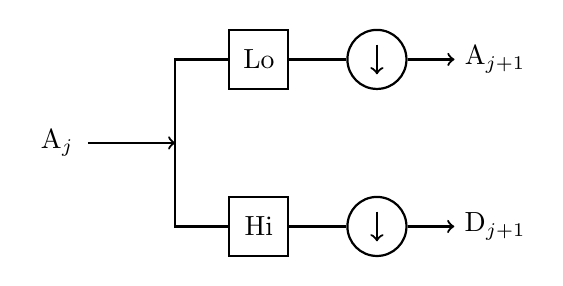
\begin{tikzpicture}[auto, node distance=1.5cm, thick, main node/.style={circle, draw}, LoHi/.style={rectangle, draw}, minimum size=.75cm]
    \node[draw=none](Aj){A$_j$};
    \node[draw=none](j1)[right of=Aj]{};
    \node[LoHi](Lo)[above right of=j1]{Lo};
    \node[LoHi](Hi)[below right of=j1]{Hi};
    \node[main node](1)[right of=Lo]{};
    \node[main node](2)[right of=Hi]{};
    \node[draw=none](Aj+1)[right of=1]{A$_{j+1}$};
    \node[draw=none](Dj+1)[right of=2]{D$_{j+1}$};

\foreach \s/\t in {Aj/j1.center, 1/Aj+1, 2/Dj+1}{
    \draw[->] (\s) -- (\t);}
\foreach \s/\t in {j1.center/Lo, j1.center/Hi}{
    \draw[](\s) |- (\t);}
\foreach \s/\t in {Lo/1, Hi/2}{
    \draw[](\s) -- (\t);}
\foreach \s in {1, 2}{
    \draw[->, shorten >=.2cm, shorten <=.2cm] (\s.north) -- (\s.south);}
\end{tikzpicture}

\vspace{1cm}

\begin{center}
\begin{tikzpicture}
% Key
    \node[draw=none, node distance=2.5cm](K)[below of=Aj]{Key:};
    \node[rectangle, draw, minimum size=.5cm, node distance=1cm](rect)[right of=K]{};
    \node[draw=none, node distance=1.3cm](conv)[right of=rect]{= convolve};
    \node[circle, draw, minimum size=.5cm, node distance=3cm](circ)[right of=rect]{};
    \node[draw=none, node distance=1.5cm](conv)[right of=circ]{= downsample};
    \draw[->, shorten >=.1cm, shorten <=.1cm] (circ.north) -- (circ.south);
\end{tikzpicture}
\end{center}
\caption{The one-dimensional discrete wavelet transform implemented as a filter bank.}
\label{fig:filter bank}
\end{figure}

\begin{comment}
At each stage of the algorithm, we filter the signal into an approximation and its details.
Note that the algorithm returns a sequence of one dimensional arrays
\[A_n, D_n, D_{n-1}, \ldots, D_1.\]
If the input signal $X$ has length $2^m$ for
some $m \geq n$ and we are using the Haar wavelet, then $A_n$ has length $2^{m-n}$, and $D_i$ has length $2^{m-i}$
for $i=1,\ldots,n$. The arrays $D_i$ are outputs of the high-pass filter, and thus represent high-frequency
details.
Hence, these arrays are known as \emph{details}.
The array $A_n$ is computed by recursively passing the signal through the low-pass filter, and hence it
represents the low-frequency structure in the signal.
In fact, $A_n$ can be seen as a smoothed approximation of the original signal, and is called the \emph{approximation}.
\end{comment}

As noted earlier, the key mathematical operations of the discrete wavelet transform are convolution and downsampling.
Given a filter and a signal, the convolution can be obtained using \li{scipy.signal.fftconvolve()}.
\begin{lstlisting}
>>> from scipy.signal import fftconvolve
>>> # Initialize a filter.
>>> L = np.ones(2)/np.sqrt(2)
>>> # Initialize a signal X.
>>> X = np.sin(np.linspace(0,2*np.pi,16))
>>> # Convolve X with L.
>>> fftconvolve(X, L)
[ -1.84945741e-16   2.87606238e-01   8.13088984e-01   1.19798126e+00
   1.37573169e+00   1.31560561e+00   1.02799937e+00   5.62642704e-01
   7.87132986e-16  -5.62642704e-01  -1.02799937e+00  -1.31560561e+00
  -1.37573169e+00  -1.19798126e+00  -8.13088984e-01  -2.87606238e-01
  -1.84945741e-16]
\end{lstlisting}

The convolution operation alone gives redundant information, so it is downsampled to keep only what is needed.
The array will be downsampled by a factor of 2, which means keeping only every other entry:

\begin{lstlisting}
>>> # Downsample an array X.
>>> sampled = X[1::2] # Keeps odd entries
\end{lstlisting}

Both the approximation and detail coefficients are computed in this manner.  The approximation uses the low-pass filter while the detail uses the high-pass filter.
Implementation of a filter bank is found in Algorithm \ref{alg:1d_wavelet}.

\begin{algorithm}[H]
\begin{algorithmic}[1]
\Procedure{dwt}{$X, L, H, n$}
    \State $A_0 \gets X$            \Comment{Initialization.}
   \For{$i=0 \ldots n-1$}
        \State $D_{i+1} \gets \,\,DS(A_i * H)$ \Comment{High-pass filter and downsample.}
        \State $A_{i+1} \gets \,\,DS(A_i * L)$ \Comment{Low-pass filter and downsample.}
    \EndFor
    \State \pseudoli{return} $A_n,D_n, D_{n-1},\ldots, D_1$.
\EndProcedure
\end{algorithmic}
\caption{The one-dimensional discrete wavelet transform. $X$ is the signal to be transformed, $L$ is the low-pass filter, $H$ is the high-pass filter and $n$ is the number of
filter bank iterations.}
\label{alg:1d_wavelet}
\end{algorithm}

\begin{problem}
Write a function that calculates the discrete wavelet transform using Algorithm \ref{alg:1d_wavelet}.
The function should return a list of one-dimensional NumPy arrays in the following form: $[A_n, D_n, \ldots, D_1]$.

%The main body of your function should be a loop in which you calculate two arrays: the $i$-th approximation
%and detail coefficients. Append the detail coefficients array to your list, and feed the approximation array
%back into the loop. When the loop is finished, append the approximation array. Finally, reverse the order of your list
%to adhere to the required return format.

Test your function by calculating the Haar wavelet coefficients of a noisy sine signal with $n=4$:

\begin{lstlisting}
domain = np.linspace(0, 4*np.pi, 1024)
noise =  np.random.randn(1024)*.1
noisysin = np.sin(domain) + noise
coeffs = dwt(noisysin, L, H, 4)
\end{lstlisting}

Plot the original signal with the approximation and detail coefficients and verify that they match the plots in Figure \ref{fig:dwt1D}.
\\ (Hint: Use array broadcasting). 

Note: the plots in your jupyter notebook \textit{do not} have to be labeled exactly like those in \ref{fig:dwt1D}. As long as the signals are clearly visible that is enough.
\label{prob:dwt1D}
\end{problem}

\begin{figure}[H]
\centering
\includegraphics[width = 0.5\textwidth]{figures/dwt1D}
\caption{A level four wavelet decomposition of a signal.
The top panel is the original signal, the next panel down is the approximation, and the remaining panels are the detail coefficients.
Notice how the approximation resembles a smoothed version of the original signal, while the details capture the high-frequency oscillations and noise.}
\label{fig:dwt1D}
\end{figure}

\subsection*{Inverse Discrete Wavelet Transform}

The process of the discrete wavelet transform is reversible.
Using modified filters, a set of detail and approximation coefficients can be manipulated and combined to recreate a signal.
The Haar wavelet filters for the inverse transformation are found by reversing the operations for each filter.
% The original lowpass filter found the average of elements, so the inverse filter will find the distance.
% The original highpass filter found the distance of elements, so the inverse filter will find the average.
The Haar inverse filters are given below:
\begin{align*}
L^{-1} &= \begin{bmatrix}\frac{\sqrt{2}}{2} & \frac{\sqrt{2}}{2}\end{bmatrix}\\H^{-1}&=\begin{bmatrix}\frac{\sqrt{2}}{2}&-\frac{\sqrt{2}}{2}\end{bmatrix}
\end{align*}
The first row refers to the inverse high-pass filter and the second row refers to the inverse low-pass filter.

Suppose the wavelet coefficients $A_n$ and $D_n$ have been computed.
$A_{n-1}$ can be recreated by tracing the schematic in Figure \ref{fig:filter bank} backwards: $A_n$ and $D_n$ are first upsampled, and then are convolved with the inverse low-pass and high-pass filters, respectively.
In the case of the Haar wavelet, \emph{upsampling} involves doubling the length of an array by inserting a 0 at every other position.
To complete the operation, the new arrays are convolved and added together to obtain $A_{n-1}$.

\begin{lstlisting}
>>> # Upsample the coefficient arrays A and D.
>>> up_A = np.zeros(2*A.size)
>>> up_A[::2] = A
>>> up_D = np.zeros(2*D.size)
>>> up_D[::2] = D
>>> # Convolve and add, discarding the last entry.
>>> A = fftconvolve(up_A, L)[:-1] + fftconvolve(up_D, H)[:-1]
\end{lstlisting}

This process is continued with the newly obtained approximation coefficients and with the next detail coefficients until the original signal is recovered.
%Now that we have $A_{n-1}$, we repeat the process with $A_{n-1}$ and $D_{n-1}$ to obtain
%$A_{n-2}$. Proceed for a total of $n$ steps (one for each $D_n, D_{n-1},\ldots ,D_1$) until we have obtained $A_0$.
%Since $A_0$ is defined to be the original
%signal, we have finished the inverse transformation.
% TODO: proof that this works, perhaps in an appendix...

\begin{problem} % Inverse wavelet transform
Write a function that performs the inverse wavelet transform.
The function should accept three things as arguments: a list of arrays (of the same form as the output of Problem \ref{prob:dwt1D}), a reverse low-pass filter, and a reverse high-pass filter.
The function should return a single array, which represents the recovered signal.

Note that the input list of arrays has length $n+1$ (consisting of $A_n$ together with $D_n, D_{n-1}, \ldots, D_1$). Your code should run once per $D_i$ matrix so it should execute a total of $n$ times.

To test your function, first perform the inverse transform on the noisy sine wave that you created in the first problem.
Then, compare the original signal with the signal recovered by your inverse wavelet transform function using \li{np.allclose()}.
\end{problem}

\begin{warn}
Although Algorithm \ref{alg:1d_wavelet} and the preceding discussion apply in the general case, the code implementations apply only to the Haar wavelet.
Because of the nature of the discrete convolution, when convolving with longer filters, the signal to be transformed needs to undergo a different type of lengthening in order to avoid
information loss during the convolution.
As such, the functions written in Problems 1 and 2 will only work correctly with the Haar filters and would require modifications to be compatible with more wavelets.
\end{warn}



\section*{The Two-dimensional Wavelet Transform} % ==============================

The generalization of the wavelet transform to two dimensions is similar to one dimensional transforms.
Again, the two primary operations used are convolution and downsampling.
The main difference in the two-dimensional case is the number of convolutions and downsamples per iteration.
First, the convolution and downsampling are performed along the rows of an array.
This results in two new arrays, as in the one dimensional case.
Then, convolution and downsampling are performed along the columns of the two new arrays.
This results in four final arrays that make up the new approximation and detail coefficients.
See Figure \ref{fig:filter bank2d}.

\begin{figure}[h]
\begin{center}
\begin{tikzpicture}[node distance=1.5cm,thick,main/.style={circle,draw}, LoHi/.style={rectangle,draw},minimum size=.75cm]

%Nodes
\node (LLj) {$LL_j$};
\node[draw=none,right of=LLj] (Aux1) {};
%First split - two layers
\node[LoHi,above right of=Aux1] (Lo1) {Lo};
\node[LoHi,below right of=Aux1] (Hi1) {Hi};
\node[main,right of=Lo1] (A1) {};
\node[main,right of=Hi1] (A2) {};
%Second split - four layers
\node[draw=none,right of=A1] (Aux2) {};
\node[draw=none,right of=A2] (Aux3) {};
\node[LoHi,right of=Aux2] (Hi2) {Hi};
\node[LoHi,right of=Aux3] (Lo3) {Lo};
\node[LoHi,below of=Lo3] (Hi3) {Hi};
\node[LoHi,above of=Hi2] (Lo2) {Lo};
\node[main,right of=Lo2] (A3) {};
\node[main,right of=Hi2] (A4) {};
\node[main,right of=Lo3] (A5) {};
\node[main,right of=Hi3] (A6) {};
\node[right of=A3] (LLj1) {$LL_{j+1}$ (A)};
\node[right of=A4] (LHj1) {$LH_{j+1}$ (H)};
\node[right of=A5] (HLj1) {$HL_{j+1}$ (V)};
\node[right of=A6] (HHj1) {$HH_{j+1}$ (D)};

\node[above right=1.6cm and -.25cm of Lo1] {$rows$};
\node[above right=.1cm and -.25cm of Lo2] {$columns$};

%Arrows between nodes
\foreach \s/\t in {LLj/Aux1.center,A3/LLj1,A4/LHj1,A5/HLj1,A6/HHj1} \draw[->,>=stealth'] (\s) -- (\t);
% |- links
\foreach \s/\t in {Aux1.center/Lo1,Aux1.center/Hi1,Aux2.center/Lo2,Aux3.center/Hi3} \draw (\s) |- (\t);
%Lines between nodes
\foreach \s/\t in {Lo1/A1,Hi1/A2,A1/Hi2,A2/Lo3,Lo2/A3,Hi2/A4,Lo3/A5,Hi3/A6} \draw (\s) -- (\t);
%Arrows in nodes
\foreach \a in {A1,A2,A3,A4,A5,A6} \draw[->,>=stealth',shorten >=.2cm,shorten <=.2cm] (\a.north) -- (\a.south);

\end{tikzpicture}

\vspace{1cm}

\begin{tikzpicture}[thick]
% Key
\node[draw=none,node distance=2.5cm] (K) [below of=LLj] {Key:};
\node[rectangle,draw,minimum size=.5cm,node distance=1cm] (rect) [right of=K] {};
\node[draw=none,node distance=1.3cm] (conv) [right of=rect] {= convolve};
\node[circle,draw,minimum size=.5cm,node distance=3cm] (circ) [right of=rect]{};
\node[draw=none,node distance=1.5cm] (conv) [right of=circ] {= downsample};
\draw[->,shorten >=.1cm,shorten <=.1cm] (circ.north) -- (circ.south);
\end{tikzpicture}

\caption{The two-dimensional discrete wavelet transform implemented as a filter bank.}
\label{fig:filter bank2d}
\end{center}
\end{figure}

When implemented as an iterative filter bank, each pass through the filter bank yields one set of approximation coefficients plus three sets of detail coefficients.
More specifically, if the two-dimensional array $X$ is the input to the filter bank, the arrays $Approx$, $H$, $V$, and $D$ are obtained.
$Approx$ is a smoothed approximation of $X$ (similar to $A_n$ in the one-dimensional case), and the other three arrays contain detail coefficients that capture high-frequency oscillations in
horizontal ($H$), vertical ($V$), and diagonal ($D$) directions.
The arrays $A$, $H$, $V$, and $D$ are known as \emph{subbands}.
Any or all of the subbands can be fed into a filter bank to further decompose the signal into additional subbands.
This decomposition can be represented by a partition of a rectangle, called a \emph{subband pattern}.
The subband pattern for one pass of the filter bank is shown in Figure \ref{fig:2dsubbands}, with an example of an image decomposition given in Figure \ref{fig:dwt2D}.

\begin{figure}[H]
\begin{tikzpicture}
%\node[draw, thick, minimum size=4cm](-2,-2) square (2,2) []{$A_k$};
\draw[thick] (-2,-2) rectangle (2,2);
\draw[step=2cm,thick,draw](4,-2) grid (8,2);
\draw[thick] (4,-2) -- (8,-2);

\node[draw=none]()at(0,0){$X$};
\node[draw=none]()at(5,1){$A$};
\node[draw=none]()at(7,1){$H$};
\node[draw=none]()at(5,-1){$V$};
\node[draw=none]()at(7,-1){$D$};
\draw[->, >=stealth', thick, shorten <=.2cm, shorten >=.2cm]
    (2,0)--(4,0);
\end{tikzpicture}
\caption{The subband pattern for one step in the 2-dimensional wavelet transform.}
\label{fig:2dsubbands}
\end{figure}

\begin{figure}[H]
% the Mandrill image used to compute these images is found at http://homepages.cae.wisc.edu/~ece533/images/ (baboon.png)
\centering
        \begin{subfigure}{0.4\textwidth}\centering
                    \includegraphics[width=\linewidth]{figures/mandrill1.png}
       \end{subfigure}%
%    \hfill
        \begin{subfigure}{0.4\textwidth}\centering
                    \includegraphics[width=\linewidth]{figures/mandrill2.png}
       \end{subfigure}%
    \hfill
        \begin{subfigure}{0.4\textwidth}\centering
                    \includegraphics[width=\linewidth]{figures/mandrill3.png}
       \end{subfigure}%
 %   \hfill
        \begin{subfigure}{0.4\textwidth}\centering
                    \includegraphics[width=\linewidth]{figures/mandrill4.png}
       \end{subfigure}
    \caption{Subbands for the mandrill image after one pass through the filter bank.
    Note how the upper left subband ($A$) is an approximation of the original Mandrill image, while the other
    three subbands highlight the stark vertical, horizontal, and diagonal changes in the image.\\
    Original image source: \url{http://sipi.usc.edu/database/}.}
    \label{fig:dwt2D}
\end{figure}

The wavelet coefficients obtained from a two-dimensional wavelet transform are used to analyze and manipulate images at differing levels of resolution.
Images are often sparsely represented by wavelets; that is, most of the image information is captured by a small subset of the wavelet coefficients.
This is a key fact for wavelet-based image compression and will be discussed in further detail later in the lab.

\section*{The PyWavelets Module} % ============================================

PyWavelets is a Python package designed for wavelet analysis.
Although it has many other uses, in this lab it will primarily be used for image manipulation.
PyWavelets can be installed using the following command:
\begin{lstlisting}
$ pip install PyWavelets
\end{lstlisting}

\begin{comment}
The most recent version of PyWavelets can be installed using the Anaconda distribution with the following code:

\begin{lstlisting}
$ conda install -c ioos pywavelets=0.4.0
\end{lstlisting}
\end{comment}

PyWavelets provides a simple way to calculate the subbands resulting from one pass through the filter bank.
The following code demonstrates how to find the approximation and detail subbands of an image.

\begin{lstlisting}
>>> from imageio import imread
>>> import pywt                             # The PyWavelets package.
# The True parameter produces a grayscale image.
>>> mandrill = imread('mandrill1.png', True)
# Use the Daubechies 4 wavelet with periodic extension.
>>> lw = pywt.dwt2(mandrill, 'db4', mode='per')
\end{lstlisting}

The function \li{pywt.dwt2()} calculates the subbands resulting from one pass through the filter bank.
The second positional argument specifies the type of wavelet to be used in the transform.
The \li{mode} keyword argument sets the extension mode, which determines the type of padding used in the convolution operation.
For the problems in this lab, always use \li{mode='per'}, which is the periodic extension.
The function \li{dwt2()} returns a tuple.
The first entry of the list is the $A$, or approximation, subband.
The second entry of the list is a separate tuple containing the remaining subbands, $H$, $V$, and $D$ (in that order).
\begin{comment}
These subbands can be plotted as follows:

\begin{lstlisting}
>>> plt.subplot(221)
>>> plt.imshow(lw[0], cmap='gray')
>>> plt.axis('off')
>>> plt.subplot(222)
# The absolute value of the detail subbands is plotted to highlight contrast.
>>> plt.imshow(np.abs(lw[1][0]), cmap='gray')
>>> plt.axis('off')
>>> plt.subplot(223)
>>> plt.imshow(np.abs(lw[1][1]), cmap='gray')
>>> plt.axis('off')
>>> plt.subplot(224)
>>> plt.imshow(np.abs(lw[1][2]), cmap='gray')
>>> plt.axis('off')
>>> plt.subplots_adjust(wspace=0, hspace=0)      # Remove space between plots.
\end{lstlisting}
\end{comment}
% As noted, the second positional argument is a string that gives the name of the wavelet to be used.

PyWavelets supports a number of different wavelets which are divided into different classes known as families.
The supported families and their wavelet instances can be listed by executing the following code:

\begin{lstlisting}
>>> # List the available wavelet families.
>>> print(pywt.families())
<<['haar', 'db', 'sym', 'coif', 'bior', 'rbio', 'dmey', 'gaus', 'mexh', 'morl', 'cgau', 'shan', 'fbsp', 'cmor']>>
>>> # List the available wavelets in a given family.
>>> print(pywt.wavelist('coif'))
<<['coif1', 'coif2', 'coif3', 'coif4', 'coif5', 'coif6', 'coif7', 'coif8', 'coif9', 'coif10', 'coif11', 'coif12', 'coif13', 'coif14', 'coif15', 'coif16', 'coif17']>>
\end{lstlisting}

It's important to note that the names from the wavelist are what we use when we call \li{dwt2}. Sometimes the name of a family will also exist as a wavelet transform in the wave list, but not always.
Different wavelets have different properties; the most suitable wavelet is dependent on the specific application.
For example, the morlet wavelet is closely related to human hearing and vision.
Note that not all of these families work with the function \li{pywt.dwt2()}, because they are continuous wavelets.
%The best wavelet to use in a particular application is rarely known beforehand.
Choosing which wavelet is used is partially based on the properties of a wavelet, but since many wavelets share desirable properties, the best wavelet for a particular application is often not known without
some type of testing.

\begin{info}
The numerical value in a wavelets name refers to the filter length.
This value is multiplied by the standard filter length of the given wavelet, resulting in the new filter length.
For example, \li{coif1} has filter length 6 and \li{coif2} has filter length 12.
\end{info}
%See Figure \ref{fig:more_wavelets} for the plots of some of additional wavelets.

\begin{comment}
\begin{figure}
\begin{subfigure}[b]{0.45\textwidth}
    \includegraphics[width=\textwidth]{figures/mexicanHat}
\end{subfigure}
\begin{subfigure}[b]{0.45\textwidth}
    \includegraphics[width=\textwidth]{figures/db5_3}
\end{subfigure}
\caption{Mexican Hat and Daubechies 4 mother wavelets.}
\label{fig:more_wavelets}
\end{figure}
\end{comment}

\begin{problem}
Explore the two-dimensional wavelet transform by completing the following:
\begin{enumerate}
    \item Save a picture of a raccoon with the following code
\begin{lstlisting}
>>> from scipy.misc import face
>>> racoon = face(True)
\end{lstlisting}
    \item Plot the subbands of raccoon as described above (using the Daubechies 4 wavelet with periodic extension).
        Compare this with the subbands of the mandrill image shown in Figure \ref{fig:dwt2D}.
    \item Compare the subband patterns of the haar, symlet, and coiflet wavelets of the raccoon picture by plotting the subbands after one pass through the filter bank.
    The haar subband should have more detail than the symlet subband, and the symlet subband should have more detail than the coiflet wavelet.
\end{enumerate}

A few Hints: for plotting, find a function that will plot an image given an array. Also, when plotting the transformations that represent the horizontal, vertical, or diagonal components of the image take \li{np.abs()} of the array when you plot it. This will radicalize the array and make its detections easier to view. Finally, you will run into an error if you try to use just \'sym\' as an arguement. Consider why this could be and how you might find the proper argument to use.
\end{problem}

The function \li{pywt.wavedec2()} is similar to \li{pywt.dwt2()}, but it also includes a keyword argument, \li{level}, which specifies the number of times to pass an image through the filter bank.
It will return a list of subbands, the first of which is the final approximation subband, while the remaining elements are tuples which contain sets of detail subbands ($H$, $V$, and $D$). For example, if I were to call pywt.wavedec2 with level=4, the output would be of the form [Approx, (H4,V4,D4),(H3,V3,D3),(H2,V2,D2),(H1,V1,D1)].

If \li{level} is not specified, the number of passes through the filter bank will be the maximum level where the decomposition is still useful.
The function \li{pywt.waverec2()} accepts a list of subband patterns (like the output of \li{pywt.wavedec2()} or \li{pywt.dwt2()}), a name string denoting the wavelet, and a keyword argument
\li{mode} for the extension mode.
It returns a reconstructed image using the reverse filter bank.
When using this function, be sure that the wavelet and mode match the deconstruction parameters.
PyWavelets has many other useful functions including \li{dwt()}, \li{idwt()} and \li{idwt2()} which can be explored further in the documentation for PyWavelets, \url{https://pywavelets.readthedocs.io/en/latest/index.html}.



\begin{comment} %A more simplified image processing technique, it works but it is very easy to implement and it is not very interesting.
If this is included in the future, consider setting the coefficients of the final detail level to 0 instead of removing them from the reconstruction.
This gives similar results without reducing the size of the image.
\section*{Image Processing}
We are now ready to use the two-dimensional wavelet transform for image processing.
Wavelets are especially good at filtering out high-frequency noise from an image.
Just as we were able to pinpoint the noise added to the sine wave in Figure \ref{fig:dwt1D}, the majority of the noise added to an image will be contained in the final $LH$, $HL$, and $HH$ detail subbands of our wavelet decomposition.
If we decompose our image and reconstruct it with all subbands except these final subbands, we will eliminate most of the troublesome noise while preserving the primary aspects of the image.

We perform this cleaning as follows:
\begin{lstlisting}
image = imread(filename,True)
wavelet = pywt.Wavelet('haar')
WaveletCoeffs = pywt.wavedec2(image,wavelet)
new_image = pywt.waverec2(WaveletCoeffs[:-1], wavelet)
\end{lstlisting}

\begin{problem}
Write a function called \li{clean_image()} which accepts the name of a grayscale image file and cleans high-frequency noise out of the image.
Load the image as an ndarray, and perform a wavelet decomposition using PyWavelets.
Reconstruct the image using all subbands except the last set of detail coefficients, and return this cleaned image as an ndarray.
\end{problem}
\end{comment}


\section*{Applications}

\subsection*{Noise Reduction}
Noise in an image is defined as unwanted visual artifacts that obscure the true image.
Images acquire noise from a variety of sources, including cameras, data transfer, and image processing algorithms.
%Noise can be completely random and incoherent (as in Figure \ref{fig:incoherent}), or it can be coherent and display visual patterns (Figure \ref{fig:coherent}).
This section will focus on reducing a particular type of noise in images called \emph{Gaussian white noise}.

%\begin{figure}[t]
%\minipage{0.49\textwidth}
%    \includegraphics[width=\linewidth]{figures/phantom_random.pdf}
%    \caption{The Phantom image with incoherent noise}
%    \label{fig:incoherent}
%\endminipage\hfill
%\minipage{0.49\textwidth}
%    \includegraphics[width=\linewidth]{figures/phantom_coherent.pdf}
%    \caption{The Phantom image with coherent noise}
%    \label{fig:coherent}
%\endminipage
%\end{figure}

Gaussian white noise causes every pixel in an image to be perturbed by a small amount. % such that the perturbations are normally distributed.
Many types of noise, including Gaussian white noise, are very high-frequency.
Since many images are relatively sparse in high-frequency domains, noise in an image can be safely removed from the high frequency subbands while minimally distorting the true image.
A basic, but effective, approach to reducing Gaussian white noise in an image is thresholding.
Thresholding can be done in two ways, referred to as hard and soft thresholding.

Given a positive threshold value $\tau$, hard thresholding sets every detail coefficient whose magnitude is less than $\tau$ to zero, while leaving the remaining coefficients untouched.
Soft thresholding also zeros out all coefficients of magnitude less than $\tau$, but in addition maps the remaining positive coefficients $\beta$ to $\beta - \tau$ and the remaining negative coefficients
$\alpha$ to $\alpha + \tau$.

\begin{comment}
Implementing these simple thresholding algorithms in Python is straight-forward, but PyWavelets already provides this functionality.
The following code gives an example.

\begin{lstlisting}
>>> A = np.arange(-4,5).reshape(3,3)
>>> A
array([[-4, -3, -2],
       [-1,  0,  1],
       [ 2,  3,  4]])
>>> pywt.thresholding.hard(A,1.5)
array([[-4, -3, -2],
       [ 0,  0,  0],
       [ 2,  3,  4]])
>>> pywt.thresholding.soft(A,1.5)
array([[-2.5, -1.5, -0.5],
       [ 0. ,  0. ,  0. ],
       [ 0.5,  1.5,  2.5]])
\end{lstlisting}
\end{comment}

Once the coefficients have been thresholded, the inverse wavelet transform is used to recover the denoised image.
%This can be done by calling the \li{waverec2} function, providing the list of Wavelet coefficients as well as the name of the desired Wavelet as arguments.
The threshold value is generally a function of the variance of the noise, and in real situations, is not known.
In fact, noise variance estimation in images is a research area in its own right, but that goes beyond the scope of this lab.

%\begin{figure}[t]
%    \includegraphics[width=\linewidth]{figures/denoise.pdf}
%    \caption{Noisy Lena (left), denoised using hard thresholding (center), and denoised using soft thresholding (right).}
%    \label{fig:denoise}
%\end{figure}

\begin{problem}
Write two functions that accept a list of wavelet coefficients in the usual form, as well as a threshold value. Each function returns the thresholded wavelet coefficients (also in the usual form). The first function should implement hard thresholding and the second should implement soft thresholding.
While writing these two functions, remember that only the detail coefficients (meaning the elements of H,V, or D arrays) are thresholded, so the first entry of the input coefficient list (The A matrix) should remain unchanged. 

To test your functions, perform hard and soft thresholding on \texttt{noisy\_darkhair.png} and plot the resulting images together.
When testing your function, use the Daubechies 4 wavelet and four sets of detail coefficients (\li{level=4} when using \li{wavedec2()}).
For soft thresholding use $\tau=20$, and for hard thresholding use $\tau=40$.

\noindent Some notes:
\begin{enumerate}
\item Masking will be helpful however it's important to consider the order in which you change values since adjusting certain values by $\tau$ initially can skew which conditions that value satisfies. Use your masks in a safe order.
\item In previous problems there was only one tuple of detail coefficients now there may be more. Make sure your code is robust enough to handle any number of tuples of detail coefficients.
\end{enumerate}
 
\end{problem}

\begin{comment}
\begin{problem}
Create a noisy version of the Lena image by adding Gaussian
white noise of mean 0 and standard deviation $\sigma = 20$ (i.e. \li{scale=20}).
Compute four levels of the wavelet coefficients using the Daubechies 4 Wavelet,
and input these into your
thresholding functions (with $\tau = 3\sigma$ for the hard threshold,
and $\tau = 3\sigma/2$ for the soft threshold). Reconstruct the
two denoised images, and then plot these together alongside the
noisy image. Your output should match Figure \ref{fig:denoise}.

What do you notice? How does lowering or raising the
threshold affect the reconstructed images? What happens if you use
a different Wavelet?
\end{problem}
\end{comment}


\subsection*{Image Compression} % ---------------------------------------------

Transform methods based on Fourier and wavelet analysis play an important role in image compression; for example, the popular JPEG image compression standard is based on the discrete cosine transform.
The JPEG2000 compression standard and the FBI Fingerprint Image database, along with other systems, take the wavelet approach.

The general framework for compression is as follows.
First, the image to be compressed undergoes some form of preprocessing, depending on the particular application.
Next, the discrete wavelet transform is used to calculate the wavelet coefficients, and these are then \emph{quantized}, i.e. mapped to a set of discrete values (for example, rounded to the nearest integer).
The quantized coefficients are then passed through an entropy encoder (such as Huffman Encoding), which reduces the number of bits required to store the coefficients.
What remains is a compact stream of bits that can be saved or transmitted much more efficiently than the original image.
The steps above are nearly all invertible (the only exception being quantization), allowing the original image to be almost perfectly reconstructed from the compressed bitstream.
See Figure \ref{tikz:wsqscheme}.

\begin{figure}[H]
\centering
\begin{tikzpicture}[rect/.style= {draw=none, node distance = 3cm},
    rect2/.style = {draw, thick, minimum width=3cm, minimum
    height=1cm}, >=stealth', shorten >=2pt]

\node[rect] (IM) [] {Image};
\node[rect2, node distance=3cm] (PR) [right of = IM]
    {Pre-Processing};
\node[rect2, node distance=4.5cm] (WD)[right of= PR]
    {Wavelet Decomposition};
\node[rect2, node distance=1.75cm](Q) [below=of PR.west, anchor=west]
    {Quantization};
\node[rect2, node distance = 1.75cm](EC)[below=of WD.west, anchor=west]
    {Entropy Coding};
\node[rect, node distance= 3.5cm](BS)[right of=EC]
    {Bit Stream};

\foreach \s/\t in {IM/PR, PR/WD, Q/EC, EC/BS}
    {\path[->, thick](\s) edge (\t);}
\draw[|-,-|,->, thick](WD.south) |-+(0,-1em)-| (Q.north);


\end{tikzpicture}
\caption{Wavelet Image Compression Schematic}
\label{tikz:wsqscheme}
\end{figure}

%\begin{comment}

\subsection*{WSQ: The FBI Fingerprint Image Compression Algorithm} % ----------

The Wavelet Scalar Quantization (WSQ) algorithm is among the first successful wavelet-based image compression algorithms.
It solves the problem of storing millions of fingerprint scans efficiently while meeting the law enforcement requirements for high image quality.
This algorithm is capable of achieving compression ratios in excess of 10-to-1 while retaining excellent image quality; see Figure \ref{fig:finger_compression}.
This section of the lab steps through a simplified version of this algorithm by writing a Python class that performs both the compression and decompression.
Differences between this simplified algorithm and the complete algorithm are found in the Additional Material section at the end of this lab.
% Also included in Additional Materials is a more thorough explanation of all the methods in the WSQ class.
Most of the methods of the class have already been implemented.
The following problems will detail the methods you will need to implement yourself.

\begin{figure}[H]
\centering
\begin{subfigure}{.32\textwidth}
  \centering
  \includegraphics[width=.7\linewidth]{figures/uncompressed_finger.png}
  \caption{Uncompressed}
\end{subfigure}%
\begin{subfigure}{.32\textwidth}
  \centering
  \includegraphics[width=.7\linewidth]{figures/compressed_finger(30comp).png}
  \caption{12:1 compressed}
\end{subfigure}%
\begin{subfigure}{.32\textwidth}
  \centering
  \includegraphics[width=.7\linewidth]{figures/compressed_finger(60comp).png}
  \caption{26:1 compressed}
\end{subfigure}
\caption{Fingerprint scan at different levels of compression.
Original image source: \url{http://www.nist.gov/itl/iad/ig/wsq.cfm}.
}
\label{fig:finger_compression}
\end{figure}

\subsubsection*{WSQ: Preprocessing}
Preprocessing in this algorithm ensures that roughly half of the new pixel values are negative, while the other half are positive, and all fall in the range $[-128,\,128]$.
The input to the algorithm is a matrix of nonnegative 8-bit integer values giving the grayscale pixel values for the fingerprint image.
The image is processed by the following formula:
\[
M' = \frac{M-m}{s},
\]
where $M$ is the original image matrix, $M'$ is the processed image, $m$ is the mean pixel value, and $s = \max\{\max(M) - m, m - \min(M)\}/128$
(here $\max(M)$ and $\min(M)$ refer to the maximum and minimum pixel values in the matrix). We've provided the code for this part of the algorithm.


\begin{comment}
To get the mean, min, and max of an array, and the max of two elements,
we use the following commands:
\begin{lstlisting}
>>> # assume we have an array M, numerical values a and b
>>> M.mean()
>>> M.max()
>>> M.min()
>>> max(a,b)
\end{lstlisting}
\end{comment}

%\begin{problem}
%Implement the preprocessing step as well as its inverse by implementing the class methods \li{pre_process()} and \li{post_process()}. You are essentially just coding the before mentioned function and its inverse.
%Each method accepts a NumPy array (the image) and returns the processed image as a %NumPy array.
%In the \li{pre_process()} method, calculate the values of $m$ and $s$ given above and store them in the class attributes \li{_m} and \li{_s}.
%\end{problem}

\subsubsection*{WSQ: Calculating the Wavelet Coefficients}
The next step in the compression algorithm is decomposing the image into subbands of wavelet coefficients.
In this implementation of the WSQ algorithm, the image is decomposed into five sets of detail coefficients (\li{level=5}) and one approximation subband, as shown in Figure \ref{fig:wavelets-subbands}.
Each of these subbands should be placed into a list in the same ordering as in Figure \ref{fig:wavelets-subbands} (another way to consider this ordering is the approximation subband followed by
each level of detail coefficients $[A, H_5, V_5, D_5, H_4, V_4,\dots ,D_1]$).

\begin{problem}
Implement the class method \li{decompose()}.
This function should accept an image to decompose and should return a list of ordered subbands.
Use the function \li{pywt.wavedec2()} with the \li{'coif1'} wavelet to obtain the subbands.
These subbands should then be ordered in a single list as described above.

Implement the inverse of the decomposition by writing the class method \li{recreate()}.
This function should accept a list of 16 subbands (ordered like the output of \li{decompose()}) and should return a reconstructed image.
Use \li{pywt.waverec2()} to reconstruct an image from the subbands.
Note that you will need to adjust the accepted list in order to adhere to the required input for \li{waverec2()}.
\end{problem}

\begin{figure}[H]
\begin{center}
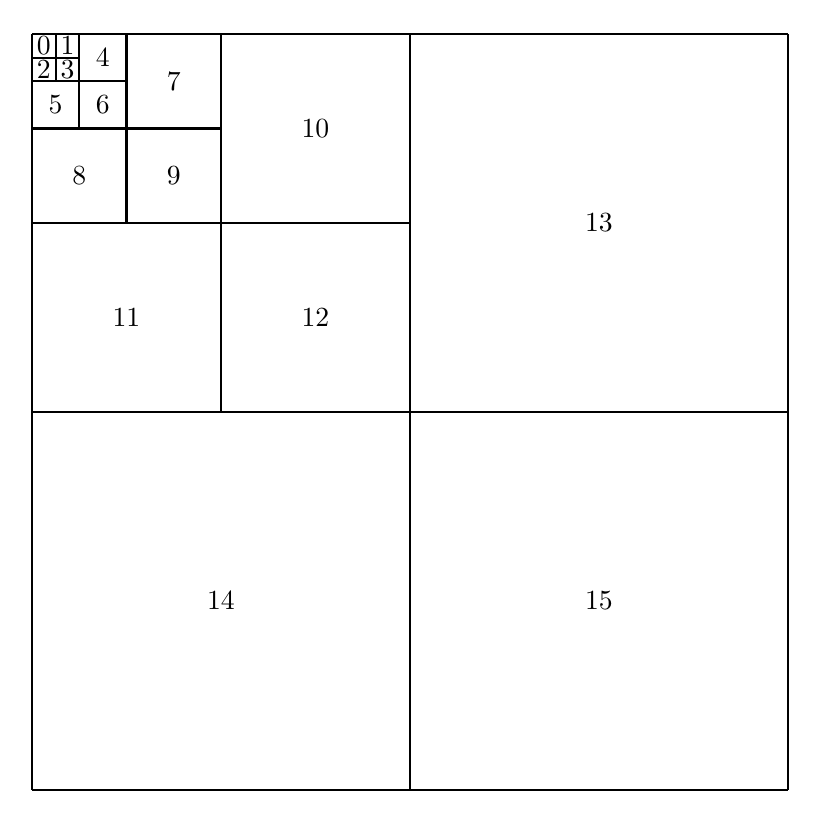
\begin{tikzpicture}[scale=.60,thick]

%Draw the grids - largest to smallest
\draw[step=8cm,draw] (0,0) grid (16,16);
\draw[step=4cm,draw] (0,8) grid (8,16);
\draw[draw,step=2cm] (0,12) grid (4,16);
\draw[draw,step=1cm] (0,14) grid (2,16);
\draw[draw,step=.5] (0,15) grid(1,16);
%Nodes for the numbers
\foreach \x/\y/\t in {.25/15.75/0,.75/15.75/1,.25/15.25/2,.75/15.25/3,1.5/15.5/4,.5/14.5/5,1.5/14.5/6,3/15/7,1/13/8,3/13/9,6/14/10,2/10/11,6/10/12,12/12/13,4/4/14,12/4/15} \node at (\x,\y) {$\t$};

\end{tikzpicture}

\caption{Subband Pattern for simplified WSQ algorithm.}
\label{fig:wavelets-subbands}
\end{center}
\end{figure}

\subsubsection*{WSQ: Quantization}
Quantization is the process of mapping each wavelet coefficient to an integer value and is the main source of compression in the algorithm.
By mapping the wavelet coefficients to a relatively small set of integer values, the complexity of the data is reduced, which allows for efficient encoding of the information in a bit string.
Further, a large portion of the wavelet coefficients will be mapped to 0 and discarded completely.
The fact that fingerprint images tend to be very nearly sparse in the wavelet domain means that little information is lost during quantization.
Care must be taken, however, to perform this quantization in a manner that achieves good compression without discarding so much information that the image cannot be accurately reconstructed.

Given a wavelet coefficient $a$ in subband $k$, the corresponding quantized coefficient $p$ is given by
\[
p =
\begin{cases}
   \left\lfloor\frac{a-Z_k/2}{Q_k}\right\rfloor + 1, & a> Z_k/2 \\
   0,       & -Z_k/2 \leq a \leq Z_k/2\\
   \left\lceil\frac{a + Z_k/2}{Q_k}\right\rceil - 1, & a < -Z_k/2,
  \end{cases}
\]
where $Z_k$ and $Q_k$ are dependent on the subband.
They determine how much compression is achieved.
If $Q_k=0$, all coefficients are mapped to 0.

An array of detail coefficients (such as $H$) can be quantized by running each value of the array through the piecewise function.

Selecting appropriate values for $Z_k$ and $Q_k$ is a tricky problem in itself, and relies on heuristics based on the statistical properties of the wavelet coefficients.
The methods that calculate these values have already been initialized.

Quantization is not a perfectly invertible process.
Once the wavelet coefficients have been quantized, some information is permanently lost.
However, wavelet coefficients $\hat{a}_k$ in subband $k$ can be roughly reconstructed from the quantized coefficients $p$ using
\[
\hat{a}_k =
\begin{cases}
(p-C)Q_k + Z_k/2, & p> 0\\
0, & p = 0\\
(p + C)Q_k - Z_k/2, & p < 0,
\end{cases}
\]
where $C$ is a new dequanitization parameter.
This process is called \emph{dequantization}.
Again, if $Q_k = 0$, $\hat{a}_k = 0$ should be returned.

\begin{problem}
Implement the quantization step by writing the \li{quantize()} method of your class.
This method should accept a NumPy array of coefficients and the quantization parameters $Q_k$ and $Z_k$.
The function should return a NumPy array of the quantized coefficients.

Also implement the \li{dequantize()} method of your class using the formula given above.
This function should accept the same parameters as \li{quantize()} as well as a parameter $C$ which defaults to $.44$.
The function should return a NumPy array of dequantized coefficients.

(Hint: Masking and array slicing will help keep your code short and fast when implementing both of these methods.
Remember the case for $Q_k=0$.
Test your functions by comparing the output of your functions to a hand calculation on a small matrix.)
%You may wish to make use of the array slicing techniques demonstrated below:
%\begin{lstlisting}
%>>> # assume X, Y are numpy arrays of same shape
%>>> m = X < -2 # create mask for entries less than -2
%>>> Y[m] = np.ceil(X[m]) + 2 # set corresponding entries of Y
%\end{lstlisting}
\end{problem}

\subsubsection*{WSQ: The Rest}
The remainder of the compression and decompression methods have already been implemented in the WSQ class.
The following discussion explains the basics of what happens in those methods.
Once all of the subbands have been quantized, they are divided into three groups.
The first group contains the smallest ten subbands (positions zero through nine), while the next two groups contain the three subbands of next largest size (positions ten through twelve and
thirteen through fifteen, respectively).
All of the subbands of each group are then flattened and concatenated with the other subbands in the group.
These three arrays of values are then mapped to Huffman indices.
Since the wavelet coefficients for fingerprint images are typically very sparse, special indices are assigned to lists of sequential zeros of varying lengths.
This allows large chunks of information to be stored as a single index, greatly aiding in compression.
The Huffman indices are then assigned a bit string representation through a Huffman map.

Python does not natively include all of the tools necessary to work with bit strings, but the Python package bitstring does have these capabilities.
Download bitstring using the following command:
\begin{lstlisting}
$ pip install bitstring
\end{lstlisting}
You will not use bitstring functions in this lab. but the code provided in the lab does call functions from the bitstring module. So you'll need to import the package with the following line of code:
\begin{lstlisting}
>>> import bitstring as bs
\end{lstlisting}


\begin{comment}
\subsubsection*{WSQ: Grouping}
At this point in the algorithm, we have a list of 64 arrays, where the $k$-th
entry is a matrix containing the quantized wavelet coefficients for the $k$-th subband.
The remaining steps in the algorithm focus on entropy coding these quantized
coefficients to further increase compression.
As such, we have finished with the wavelet analysis portion.

We will segment the list of quantized subbands into three groups.
This gives three lists of quantized coefficients, each having a high degree of homogeneity.
This is important for the entropy coding, since we can achieve better compression by separately encoding groups of similar coefficients.

Group quantized subbands $0$ through $18$ together, $19$ through $51$ together, and finally $52$ through $63$ together.
You may understand the logic of these groupings when glancing back at Figure \ref{fig:wavelets-subbands2}.
When grouping subbands together, flatten each subband and concatenate their entries together, so that you obtain a simple list of integer values.
Since we are flattening and then concatenating the subbands, we need to save the shape of the original subbands, so that we can later
reconstruct the subbands from the groups of coefficients.
Finally, we will not include subbands that consist entirely of zeros, as these contain no information and thus don't need to be stored.
Therefore, while looping through the subbands and creating the lists of coefficients, include a check for nonzero entries in the subband,
and also create a list of boolean values for each group whose $i$-th entry indicates whether the $i$-th subband in the group was included.

Below is sample code for producing the first group.
Use a similar approach for the other two groups.
\begin{lstlisting}
>>> # assume subbands is my list of the 64 quantized subbands
>>> g1 = []     # this will hold the group 1 coefficients
>>> s1 = []     # keep track of the subband dimensions in group 1
>>> t1 = []     # keep track of which subbands were included
>>> for i in xrange(19):
>>>     s1.append(subbands[i].shape)
>>>     if subbands[i].any(): # True if any nonzero entry
>>>         g1.extend(subbands[i].ravel())
>>>         t1.append(True)
>>>     else: # the subband was not transmitted
>>>         t1.append(False)
\end{lstlisting}

To reconstruct the subbands from \li{g1}, \li{s1}, and \li{t1}, we have the following code:
\begin{lstlisting}
>>> # reconstruct the subbands in group 1
>>> subbands1 = []     # the reconstructed subbands in group 1
>>> i = 0
>>> for j, shape in enumerate(s1):
>>>     if t1[j]: # if the j-th subband was included
>>>         l = shape[0]*shape[1] # number of entries in the subband
>>>         subbands1.append(np.array(g1[i:i+l]).reshape(shape))
>>>         i += l
>>>     else: # the j-th subband wasn't included, so all zeros
>>>         subbands1.append(np.zeros(shape))
\end{lstlisting}
\begin{problem}
Carry out the grouping procedure and its inverse as described above by implementing the li\{_group} and \li{ungroup} class methods:

Note that we need the shapes and the boolean lists indicating which subbands were included
for the un-grouping step.
Thus, in the \li{compress} method, once we computed these tuples of lists, we store them in the class attributes \li{_shapes}
and \li{_tvals}, respectively.
\begin{lstlisting}
>>> groups, self._shapes, self._tvals = self._group(q_subbands)
\end{lstlisting}
\end{problem}

\subsubsection*{WSQ: From Quantized Coefficients to Huffman Indices}
We now have three groups of integer-valued quantized coefficients.
It remains to encode each of these three groups using Huffman coding.

Note that each group is likely to contain many consecutive zeros, since we have rounded all of the smallest wavelet coefficients to zero.
There will also be a few quantized coefficients of high magnitude.
The remaining nonzero coefficients will have values between $-73$ and $74$.
With this in mind, we can represent these groups of coefficients even more tersely by mapping them to a set of discrete values (integers from $0$ to $253$), which we call \emph{Huffman Indices}.
The mapping between Huffman indices and quantized coefficients is given in Table \ref{table:huffIndex}.
\begin{table}
\begin{tabular}{|c|c|}
\hline
\textbf{Huffman Index} & \textbf{Quantized Coefficient}\\\hline
0 & zero run length 1\\\hline
1 & zero run length 2\\\hline
\vdots & \vdots\\\hline
99 & zero run length 100\\\hline
100 & $75\leq q \leq 255$\\\hline
101 & $-255 \leq q \leq -74$\\\hline
102 & $256 \leq q \leq 65535$\\\hline
103 & $-65535 \leq q \leq -256$\\\hline
104 & zero run of length $101\leq n \leq 255$\\\hline
105 & zero run of length $255\leq n \leq 65535$\\\hline
106 & -73\\\hline
107 & -72\\\hline
108 & -71\\\hline
\vdots & \vdots\\\hline
179 & 0 \emph{(use index 0)}\\\hline
\vdots & \vdots \\\hline
252 & 73\\\hline
253 & 74\\\hline
\end{tabular}
\caption{The mapping between Huffman indices and quantized coefficients.}
\label{table:huffIndex}
\end{table}

To see how this mapping works, suppose that we have the following list of quantized coefficients:
\[
[0, 0, 0, 0, -45, 13, 103, -269, 0]
\]
The list starts off with a zero run of length $4$, so the first Huffman index is $3$ (each zero run of length $n$ where $n\leq 100$ get a Huffman index of $n-1$).
The next coefficient is $-45$, so we infer from the Table that its Huffman index is $-45 + (106+73) = 134$.
The next coefficient is $13$, so as before, its Huffman index is $13 + 179 = 192$.
The final three indices are $100$, $103$, and $0$.

Note that this mapping is not one-to-one when dealing with zero runs of lengths greater than $100$, or with coefficients of sufficiently large magnitudes (the Huffman indices for these cases are 100 through 105).
We refer to these cases as \emph{exceptional cases}.
When we encounter exceptional cases, we need to store the length of the zero run or the magnitude of the coefficient, so that we can perfectly reconstruct the quantized coefficients at the decompression stage.
Hence, while generating a list of the Huffman indices for each group, we also generate a list of extra values for the exceptional cases.

Finally, as we generate the list of Huffman indices from the quantized coefficients, we also tabulate the frequency of each index, as this is necessary when building a Huffman Encoder.

\begin{problem}
Examine the code for \li{_huffmanIndices} to make sure you understand it, and add it to your class.
\end{problem}

In the decompression stage, we need to recover the quantized coefficients from the Huffman Indices.
As noted before, the mapping is not one-to-one for the exceptional cases, so we need both the list of indices and the extra values.
Given these two lists, it is not difficult to recover the coefficients.

\begin{problem}
Examine the code for \li{_indicesToCoeffs} for understanding, and then add the method to your class.
\end{problem}

\subsubsection*{Reading and Writing Bits with bitstring}
In the final stage of the algorithm, we take our lists of Huffman indices and map them to bit patterns.
Pure Python is not equipped to manipulate data at the bit level, so we will use the Python package \li{bitstring} to facilitate the process.
In this section we present the functions required for the WSQ algorithm.

Once you have installed the package, type the import command:
\begin{lstlisting}
>>> import bitstring as bs
\end{lstlisting}
In order to build a string of bits, we initialize a \li{BitArray} object, and then add the desired bit patterns.
\begin{lstlisting}
>>> bits = bs.BitArray()
>>> # add bit patterns 1101 and 01
>>> bits.append('0b1101')
>>> bits.append('0b01')
\end{lstlisting}
Note that the string containing the bit pattern must begin with \li{'0b'}.

We can add an 8- or 16-bit representations of an integer as follows:
\begin{lstlisting}
>>> # add the 8-bit integer 212, and then the 16-bit integer 1047
>>> bits.append('uint:8=212')
>>> bits.append('uint:16=1047')
\end{lstlisting}
To view the bits contained in the \li{BitArray}, we can print the \li{bin} attribute.
\begin{lstlisting}
>>> # view the entire bit string
>>> print bits.bin
110101110101000000010000010111
\end{lstlisting}

When reading the data from a bit stream, we use a \li{bs.ConstBitStream} object, and call its \li{read} method, giving it an input string that specifies the way to interpret the bits, and the number of bits to read.
To read the next 3 bits as binary, the input string would be \li{'bin:3'}, whereas to read the next 16 bits as an unsigned integer you would provide the input string \li{'uint:16'}.
Let's read the first 6 bits of \li{bits}, one at a time:
\begin{lstlisting}
>>> bitreader = bs.ConstBitStream(bits)
>>> for i in xrange(6):
>>>     print bitreader.read('bin:1')
1
1
0
1
0
1
\end{lstlisting}
We know that the next 8 bits should be interpreted as an unsigned integer, and likewise for the
following 16 bits. Thus, we read these bits as follows:
\begin{lstlisting}
>>> print bitreader.read('uint:8')
212
>>> print bitreader.read('uint:16')
1047
\end{lstlisting}

You now have all the tools necessary to read and write the compressed image bit stream.

\subsubsection*{WSQ: Huffman Coding}
Huffman coding is a technique for assigning binary codes to a collection of symbols in such a way that minimizes the total number of bits needed to encode the symbols.
More frequent symbols will be assigned shorter binary codes, while rare symbols will have longer codes.
One simple way to implement Huffman Coding is to build a binary tree, whose leaves correspond to the different symbols to be encoded.
We then traverse the tree from the root down to each leaf node to generate the binary codes (left corresponds to 0, right corresponds to 1).
The provided classes and functions \li{huffmanLeaf()}, \li{huffmanNode()} and \li{huffman()} implement this.


When we pass a list of Huffman indices to the function \li{huffman()}, we obtain obtain a dictionary (called the Huffman map) whose keys are the integers 0 through 253 (the Huffman indices)
and whose values are the bit pattern assigned to each Huffman index.
This Huffman map, together with the list of Huffman indices and extra values, allows us to encode the quantized coefficients as a bit string.

\begin{problem}
Add the \li{_encode()} method to your class.
Implement the Huffman coding step in the \li{compress} method by calculating the Huffman indices, Huffman map, and bit string for each group of quantized coefficients separately.
Store the resulting three bit strings and Huffman maps in the class attributes \li{_bitstrings} and \li{_huff_maps}.
Use the following code block as a guide.
\begin{lstlisting}
>>> # assume groups is a list of the three groups of coefficients
>>> # for each group, get huffman indices, create huffman tree, and encode
>>> huff_maps = []
>>> bitstrings = []
>>> for i in xrange(3):
>>>     inds, freqs, extra = self._huffmanIndices(groups[i])
>>>     huff_map = huffman(freqs)
>>>     huff_maps.append(huff_map)
>>>     bitstrings.append(self._encode(inds, extra, huff_map))
>>>
>>> # store the bitstrings and the huffman maps
>>> self._bitstrings = bitstrings
>>> self._huff_maps = huff_maps
\end{lstlisting}
You have now fully implemented the compression algorithm!
\end{problem}

For decompression, we need to decode the bit strings back to Huffman indices.
This is straight-forward enough using the Huffman maps.
Essentially, we read the bit string one bit at a time, check to see if we have a bit pattern found in the Huffman map, and if so, store the corresponding Huffman index in the list of Huffman indices.
If the Huffman index is an exceptional case, we read the next 8 or 16 bits from the bit string (depending on the exact value of the index), and store the resulting value in the list of extra values.
Examine the implementation below for understanding:

\begin{problem}
Add the \li{_decode()} method to your class.
\end{problem}

\subsubsection*{WSQ: Decompression}
Decompression refers to recovering the original image from the bit encodings of the quantized wavelet coefficients.
You already have all of the methods required for decompression; what remains is to put them together.
\begin{problem}
Add the \li{decompress()} method to your class.
\end{problem}
\end{comment}

\subsubsection*{WSQ: Calculating the Compression Ratio}
The methods of compression and decompression are now fully implemented. The final task is to verify how much compression has taken place.
The compression ratio is the ratio of the number of bits in the original image to the number of bits in the encoding.
Assuming that each pixel of the input image is an 8-bit integer, the number of bits in the original image is just eight times the number of pixels
(the number of pixels in the original source image is stored in the class attribute \li{_pixels}).
The number of bits in the encoding can be calculated by adding up the lengths of each of the three bit strings stored in the class attribute \li{_bitstrings}.
\begin{problem}
Implement the method \li{get_ratio()} by calculating the ratio of compression.
The function should not accept any parameters and should return the compression ratio.

Your compression algorithm is now complete! Test your class with the following code.
The compression ratio should be approximately 18.
\begin{lstlisting}
# Try out different values of r between .1 to .9.
r = .5
finger = imread('uncompressed_finger.png', True)
wsq = WSQ()
wsq.compress(finger, r)
print(wsq.get_ratio())
new_finger = wsq.decompress()
plt.subplot(211)
plt.imshow(finger, cmap=plt.cm.Greys_r)
plt.subplot(212)
plt.imshow(np.abs(new_finger), cmap=plt.cm.Greys_r)
plt.show()
\end{lstlisting}
\end{problem}
\newpage

\section*{Additional Material} %-------------------------------------------------------------------------------------------------------------------------------------------------------------------------------------------
%---------------------------------------------------------------------------------------------------------------------------------------------------------------------------------------------------------------------------------
\subsection*{Haar Wavelet Transform}
The Haar Wavelet Transform is a general matrix transform used to convolve Haar Wavelets.
It is found by combining the convolution matrices for a lowpass and highpass filter such that one is directly on top of the other.
The lowpass filter is taking the average of every two elements in an array and the highpass filter is taking the difference of every two elements in an array.
Redundant information given in the new matrix is then removed via downsampling.
However, in order for the transform matrix to have the property $A^T=A^{-1}$, the columns of the matrix must be normalized.
Thus, each column is normalized (and subsequently the filters) and the resulting matrix is the Haar Wavelet Transform.

For more on the Haar Wavelet Transform, see \emph{Discrete Wavelet Transformations: An Elementary Approach with Applications} by Patrick J. Van Fleet.

\subsection*{WSQ Algorithm}
The official standard for the WSQ algorithm is slightly different from the version implemented in this lab.
One of the largest differences is the subband pattern that is used in the official algorithm; this pattern is demonstrated in Figure \ref{fig:wavelets-subbands2}.
The pattern used may seem complicated and somewhat arbitrary, but it is used because of the relatively good empirical results when used in compression.
This pattern can be obtained by performing a single pass of the 2-dimensional filter bank on the image then passing each of the resulting subbands through the filter bank resulting in 16 total subbands.
This same process is then repeated with the $A$, $H$ and $V$ subbands of the original approximation subband creating 46 additional subbands.
Finally, the subband corresponding to the top left of Figure \ref{fig:wavelets-subbands2} should be passed through the 2-dimensional filter bank a single time.

\begin{comment}
We need to calculate the subband pattern found in Figure \ref{fig:wavelets-subbands2}.
This subband pattern is somewhat arbitrary, but is used because of its empirically good results in compression.
While the pattern may appear complicated at first, we can obtain the required subband coefficients rather easily.
To start, decompose the image into 16 subbands, first by using the \li{dwt2} function to split the image into four subbands, and then applying the function again to each of the four subbands.

Using the function \li{_decompose16} on the fingerprint image, you should now have a grid of 16 subbands.
Next, split each of the three subbands found in the top left corner of the subband grid into 16 additional subbands, in the same way as before.
You now have a grid of $13 + 3(16) = 61$ subbands.

Finally, take the very top left subband, and split this into four additional subbands.
You should have 64 subbands. Place them into a list in the order indicated by the numbers in Figure \ref{fig:wavelets-subbands2}.
\end{comment}

As in the implementation given above, the subbands of the official algorithm are divided into three groups.
The subbands 0 through 18 are grouped together, as are 19 through 51 and 52 through 63.
The official algorithm also uses a wavelet specialized for image compression that is not included in the PyWavelets distribution.
There are also some slight modifications made to the implementation of the discrete wavelet transform that do not drastically affect performance.

\begin{figure}[H]
\centering
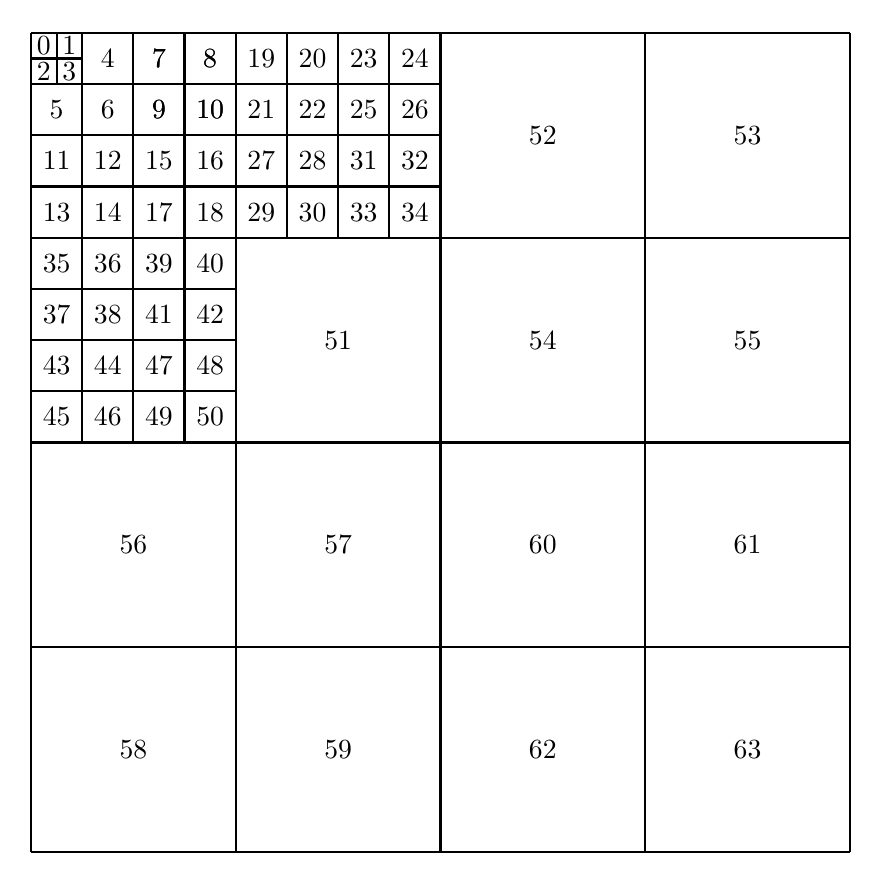
\begin{tikzpicture}[scale=.65]
\draw [draw, step=1cm, thick] (0,8) grid (4,12);
\draw[draw, thick, step=1cm] (0,12) grid (8,16);
\draw[step=4cm, thick, draw](0,0) grid (16,16);
\draw[draw, step=.5,thick](0,15)grid(1,16);

\foreach \x in {0, 1} {
  \foreach \y [evaluate=\y as \r using int((\x)+2*(\y))] in {0, 1}{
    \node[draw=none]()at(.25+.5*\x,15.75-.5*\y){\r};}}

\node[draw=none]()at(1.5, 15.5){4};
\node[draw=none]()at(.5,14.5){5};
\node[draw=none]()at(1.5,14.5){6};


\foreach \x in {0, 1} {
  \foreach \y [evaluate=\y as \r using int((\x)+2*(\y) + 7)] in {0, 1}{
    \node[draw=none]()at(2.5+1*\x,15.5-1*\y){\r};}}

\foreach \x in {0, 1} {
  \foreach \y [evaluate=\y as \r using int((\x)+2*(\y) + 7)] in {0, 1}{
    \node[draw=none]()at(2.5+1*\x,15.5-1*\y){\r};}}

\foreach \x in {0, 1} {
  \foreach \y [evaluate=\y as \r using int((\x)+2*(\y) + 11)] in {0, 1}{
    \node[draw=none]()at(.5+1*\x,13.5-1*\y){\r};}}

\foreach \x in {0, 1} {
  \foreach \y [evaluate=\y as \r using int((\x)+2*(\y) + 15)] in {0, 1}{
    \node[draw=none]()at(2.5+1*\x,13.5-1*\y){\r};}}

\foreach \j in {0, 1} {
  \foreach \k in {0, 1} {
    \foreach \x in {0, 1} {
      \foreach \y [evaluate=\y as \r using int((\x)+2*(\y) + 4*(\j) + 8*(\k)+ 19)] in {0, 1}{
        \node[draw=none]()at(4.5+2*\j+1*\x,15.5-2*\k-1*\y){\r};}}}}

\foreach \j in {0, 1} {
  \foreach \k in {0, 1} {
    \foreach \x in {0, 1} {
      \foreach \y [evaluate=\y as \r using int((\x)+2*(\y) + 4*(\j) + 8*(\k)+ 35)] in {0, 1}{
        \node[draw=none]()at(.5+2*\j+1*\x,11.5-2*\k-1*\y){\r};}}}}

\node[draw=none]()at(6,10){51};

\foreach \x in {0, 1} {
  \foreach \y [evaluate=\y as \r using int((\x)+2*(\y) + 60)] in {0, 1}{
    \node[draw=none]()at(10+4*\x,6-4*\y){\r};}}

\foreach \x in {0, 1} {
  \foreach \y [evaluate=\y as \r using int((\x)+2*(\y) + 56)] in {0, 1}{
    \node[draw=none]()at(2+4*\x,6-4*\y){\r};}}

\foreach \x in {0, 1} {
  \foreach \y [evaluate=\y as \r using int((\x)+2*(\y) + 52)] in {0, 1}{
    \node[draw=none]()at(10+4*\x,14-4*\y){\r};}}

\end{tikzpicture}
\caption{True subband pattern for WSQ algorithm.}
\label{fig:wavelets-subbands2}
\end{figure}

\begin{comment}
The following code box contains the partially implemented WSQ class that is needed to complete the problems in this lab.
\begin{lstlisting}
class WSQ:
    """Perform image compression using the Wavelet Scalar Quantization
    algorithm. This class is a structure for performing the algorithm, to
    actually perform the compression and decompression, use the _compress
    and _decompress methods respectively. Note that all class attributes
    are set to None in __init__, but their values are initialized in the
    compress method.

    Attributes:
        _pixels (int): Number of pixels in source image.
        _s (float): Scale parameter for image preprocessing.
        _m (float): Shift parameter for image preprocessing.
        _Q ((16, ), ndarray): Quantization parameters q for each subband.
        _Z ((16, ), ndarray): Quantization parameters z for each subband.
        _bitstrings (list): List of 3 BitArrays, giving bit encodings for
            each group.
        _tvals (tuple): Tuple of 3 lists of bools, indicating which
            subbands in each groups were encoded.
        _shapes (tuple): Tuple of 3 lists of tuples, giving shapes of each
            subband in each group.
        _huff_maps (list): List of 3 dictionaries, mapping huffman index to
            bit pattern.
    """

    def __init__(self):
        self._pixels = None
        self._s = None
        self._m = None
        self._Q = None
        self._Z = None
        self._bitstrings = None
        self._tvals = None
        self._shapes= None
        self._huff_maps = None
        self._infoloss = None

    def compress(self, img, r, gamma=2.5):
        """The main compression routine. It computes and stores a bitstring
        representation of a compressed image, along with other values
        needed for decompression.

        Parameters:
            img ((m,n), ndarray): Numpy array containing 8-bit integer
                pixel values.
            r (float): Defines compression ratio. Between 0 and 1, smaller
                numbers mean greater levels of compression.
            gamma (float): A parameter used in quantization.
        """
        self._pixels = img.size   # Store image size.
        # Process then decompose image into subbands.
        mprime = self.pre_process(img)
        subbands = self.decompose(img)
        # Calculate quantization parameters, quantize the image then group.
        self._Q, self._Z = self.get_bins(subbands, r, gamma)
        q_subbands = [self.quantize(subbands[i],self._Q[i],self._Z[i])
                      for i in range(16)]
        groups, self._shapes, self._tvals = self.group(q_subbands)

        # Complete the Huffman encoding and transfer to bitstring.
        huff_maps = []
        bitstrings = []
        for i in range(3):
            inds, freqs, extra = self.huffman_indices(groups[i])
            huff_map = huffman(freqs)
            huff_maps.append(huff_map)
            bitstrings.append(self.encode(inds, extra, huff_map))

        # Store the bitstrings and the huffman maps.
        self._bitstrings = bitstrings
        self._huff_maps = huff_maps

    def pre_process(self, img):
        """Preprocessing routine that takes an image and shifts it so that
        roughly half of the values are on either side of zero and fall
        between -128 and 128.

        Parameters:
            img ((m,n), ndarray): Numpy array containing 8-bit integer
                pixel values.

        Returns:
            ((m,n), ndarray): Processed numpy array containing 8-bit
                integer pixel values.
        """
        pass

    def post_process(self, img):
        """Postprocess routine that reverses pre_process().

        Parameters:
            img ((m,n), ndarray): Numpy array containing 8-bit integer
                pixel values.

        Returns:
            ((m,n), ndarray): Unprocessed numpy array containing 8-bit
                integer pixel values.
        """
        pass

    def decompose(self, img):
        """Decompose an image into the WSQ subband pattern using the
        Coiflet1 wavelet.

        Parameters:
            img ((m,n) ndarray): Numpy array holding the image to be
                decomposed.

        Returns:
            subbands (list): List of 16 numpy arrays containing the WSQ
                subbands in order.
        """
        pass

    def recreate(self, subbands):
        """Recreate an image from the 16 WSQ subbands.

        Parameters:
            subbands (list): List of 16 numpy arrays containing the WSQ
                subbands in order.

        Returns:
            img ((m,n) ndarray): Numpy array, the image recreated from the
                WSQ subbands.
        """
        pass

    def get_bins(self, subbands, r, gamma):
        """Calculate quantization bin widths for each subband. These will
        be used to quantize the wavelet coefficients.

        Parameters:
            subbands (list): List of 16 WSQ subbands.
            r (float): Compression parameter, determines the degree of
                compression.
            gamma(float): Parameter used in compression algorithm.

        Returns:
            Q ((16, ) ndarray): Array of quantization step sizes.
            Z ((16, ) ndarray): Array of quantization coefficients.
        """
        subband_vars = np.zeros(16)
        fracs = np.zeros(16)

        for i in range(len(subbands)): # Compute subband variances.
            X,Y = subbands[i].shape
            fracs[i]=(X*Y)/(np.float(finger.shape[0]*finger.shape[1]))
            x = np.floor(X/8.).astype(int)
            y = np.floor(9*Y/32.).astype(int)
            Xp = np.floor(3*X/4.).astype(int)
            Yp = np.floor(7*Y/16.).astype(int)
            mu = subbands[i].mean()
            sigsq = (Xp*Yp-1.)**(-1)*((subbands[i][x:x+Xp, y:y+Yp]-mu)**2).sum()
            subband_vars[i] = sigsq

        A = np.ones(16)
        A[13], A[14] = [1.32]*2

        Qprime = np.zeros(16)
        mask = subband_vars >= 1.01
        Qprime[mask] = 10./(A[mask]*np.log(subband_vars[mask]))
        Qprime[:4] = 1
        Qprime[15] = 0

        K = []
        for i in range(15):
            if subband_vars[i] >= 1.01:
                K.append(i)

        while True:
            S = fracs[K].sum()
            P = ((np.sqrt(subband_vars[K])/Qprime[K])**fracs[K]).prod()
            q = (gamma**(-1))*(2**(r/S-1))*(P**(-1./S))
            E = []
            for i in K:
                if Qprime[i]/q >= 2*gamma*np.sqrt(subband_vars[i]):
                    E.append(i)
            if len(E) > 0:
                for i in E:
                    K.remove(i)
                continue
            break

        Q = np.zeros(16) # Final bin widths.
        for i in K:
            Q[i] = Qprime[i]/q
        Z = 1.2*Q

        return Q, Z

    def quantize(self, coeffs, Q, Z):
        """Implementation of a uniform quantizer which maps wavelet
        coefficients to integer values using the quantization parameters
        Q and Z.

        Parameters:
            coeffs ((m,n) ndarray): Contains the floating-point values to
                be quantized.
            Q (float): The step size of the quantization.
            Z (float): The null-zone width (of the center quantization bin).

        Returns
            out ((m,n) ndarray): Numpy array of the quantized values.
        """
        pass

    def dequantize(self, coeffs, Q, Z, C=0.44):
        """Given quantization parameters, approximately reverses the
        quantization effect carried out in quantize().

        Parameters:
            coeffs ((m,n) ndarray): Array of quantized coefficients.
            Q (float): The step size of the quantization.
            Z (float): The null-zone width (of the center quantization bin).
            C (float): Centering parameter, defaults to .44.

        Returns:
            out ((m,n) ndarray): Array of dequantized coefficients.
        """
        pass

    def group(self, subbands):
        """Split the quantized subbands into 3 groups.

        Parameters:
            subbands (list): Contains 16 numpy arrays which hold the
                quantized coefficients.

        Returns:
            gs (tuple): (g1,g2,g3) Each gi is a list of quantized coeffs
                for group i.
            ss (tuple): (s1,s2,s3) Each si is a list of tuples which
                contain the shapes for group i.
            ts (tuple): (s1,s2,s3) Each ti is a list of bools indicating
                which subbands were included.
        """
        g1 = [] # This will hold the group 1 coefficients.
        s1 = [] # Keep track of the subband dimensions in group 1.
        t1 = [] # Keep track of which subbands were included.
        for i in range(10):
            s1.append(subbands[i].shape)
            if subbands[i].any(): # True if there is any nonzero entry.
                g1.extend(subbands[i].ravel())
                t1.append(True)
            else: # The subband was not transmitted.
                t1.append(False)

        g2 = [] # This will hold the group 2 coefficients.
        s2 = [] # Keep track of the subband dimensions in group 2.
        t2 = [] # Keep track of which subbands were included.
        for i in range(10, 13):
            s2.append(subbands[i].shape)
            if subbands[i].any(): # True if there is any nonzero entry.
                g2.extend(subbands[i].ravel())
                t2.append(True)
            else: # The subband was not transmitted.
                t2.append(False)

        g3 = [] # This will hold the group 3 coefficients.
        s3 = [] # Keep track of the subband dimensions in group 3.
        t3 = [] # Keep track of which subbands were included.
        for i in range(13,16):
            s3.append(subbands[i].shape)
            if subbands[i].any(): # True if there is any nonzero entry.
                g3.extend(subbands[i].ravel())
                t3.append(True)
            else: # The subband was not transmitted.
                t3.append(False)

        return (g1,g2,g3), (s1,s2,s3), (t1,t2,t3)

    def ungroup(self, gs, ss, ts):
        """Re-create the subband list structure from the information stored
        in gs, ss and ts.

        Parameters:
            gs (tuple): (g1,g2,g3) Each gi is a list of quantized coeffs
                for group i.
            ss (tuple): (s1,s2,s3) Each si is a list of tuples which
                contain the shapes for group i.
            ts (tuple): (s1,s2,s3) Each ti is a list of bools indicating
                which subbands were included.

        Returns:
            subbands (list): Contains 16 numpy arrays holding quantized
                coefficients.
        """
        subbands1 = [] # The reconstructed subbands in group 1.
        i = 0
        for j, shape in enumerate(ss[0]):
            if ts[0][j]: # True if the j-th subband was included.
                l = shape[0]*shape[1] # Number of entries in the subband.
                subbands1.append(np.array(gs[0][i:i+l]).reshape(shape))
                i += l
            else: # The j-th subband wasn't included, so all zeros.
                subbands1.append(np.zeros(shape))

        subbands2 = [] # The reconstructed subbands in group 2.
        i = 0
        for j, shape in enumerate(ss[1]):
            if ts[1][j]: # True if the j-th subband was included.
                l = shape[0]*shape[1] # Number of entries in the subband.
                subbands2.append(np.array(gs[1][i:i+l]).reshape(shape))
                i += l
            else: # The j-th subband wasn't included, so all zeros.
                subbands2.append(np.zeros(shape))

        subbands3 = [] # the reconstructed subbands in group 3
        i = 0
        for j, shape in enumerate(ss[2]):
            if ts[2][j]: # True if the j-th subband was included.
                l = shape[0]*shape[1] # Number of entries in the subband.
                subbands3.append(np.array(gs[2][i:i+l]).reshape(shape))
                i += l
            else: # The j-th subband wasn't included, so all zeros.
                subbands3.append(np.zeros(shape))

        subbands1.extend(subbands2)
        subbands1.extend(subbands3)
        return subbands1

    def huffman_indices(self, coeffs):
        """Calculate the Huffman indices from the quantized coefficients.

        Parameters:
            coeffs (list): Integer values that represent quantized
                coefficients.

        Returns:
            inds (list): The Huffman indices.
            freqs (ndarray): Array whose i-th entry gives the frequency of
                index i.
            extra (list): Contains zero run lengths and coefficient
                magnitudes for exceptional cases.
        """
        N = len(coeffs)
        i = 0
        inds = []
        extra = []
        freqs = np.zeros(254)

        # Sweep through the quantized coefficients.
        while i < N:

            # First handle zero runs.
            zero_count = 0
            while coeffs[i] == 0:
                zero_count += 1
                i += 1
                if i >= N:
                    break

            if zero_count > 0 and zero_count < 101:
                inds.append(zero_count - 1)
                freqs[zero_count - 1] += 1
            elif zero_count >= 101 and zero_count < 256: # 8 bit zero run.
                inds.append(104)
                freqs[104] += 1
                extra.append(zero_count)
            elif zero_count >= 256: # 16 bit zero run.
                inds.append(105)
                freqs[105] += 1
                extra.append(zero_count)
            if i >= N:
                break

            # now handle nonzero coefficients
            if coeffs[i] > 74 and coeffs[i] < 256: # 8 bit pos coeff.
                inds.append(100)
                freqs[100] += 1
                extra.append(coeffs[i])
            elif coeffs[i] >= 256: # 16 bit pos coeff.
                inds.append(102)
                freqs[102] += 1
                extra.append(coeffs[i])
            elif coeffs[i] < -73 and coeffs[i] > -256: # 8 bit neg coeff.
                inds.append(101)
                freqs[101] += 1
                extra.append(abs(coeffs[i]))
            elif coeffs[i] <= -256: # 16 bit neg coeff.
                inds.append(103)
                freqs[103] += 1
                extra.append(abs(coeffs[i]))
            else: # Current value is a nonzero coefficient in the range [-73, 74].
                inds.append(179 + coeffs[i])
                freqs[179 + coeffs[i].astype(int)] += 1
            i += 1

        return list(map(int,inds)), list(map(int,freqs)), list(map(int,extra))

    def indices_to_coeffs(self, indices, extra):
        """Calculate the coefficients from the Huffman indices plus extra
        values.

        Parameters:
            indices (list): List of Huffman indices.
            extra (list): Indices corresponding to exceptional values.

        Returns:
            coeffs (list): Quantized coefficients recovered from the indices.
        """
        coeffs = []
        j = 0 # Index for extra array.

        for s in indices:
            if s < 100: # Zero count of 100 or less.
                coeffs.extend(np.zeros(s+1))
            elif s == 104 or s == 105: # Zero count of 8 or 16 bits.
                coeffs.extend(np.zeros(extra[j]))
                j += 1
            elif s in [100, 102]: # 8 or 16 bit pos coefficient.
                coeffs.append(extra[j]) # Get the coefficient from the extra list.
                j += 1
            elif s in [101, 103]: # 8 or 16 bit neg coefficient.
                coeffs.append(-extra[j]) # Get the coefficient from the extra list.
                j += 1
            else: # Coefficient from -73 to +74.
                coeffs.append(s-179)
        return coeffs

    def encode(self, indices, extra, huff_map):
        """Encodes the indices using the Huffman map, then returns
        the resulting bitstring.

        Parameters:
            indices (list): Huffman Indices.
            extra (list): Indices corresponding to exceptional values.
            huff_map (dict): Dictionary that maps Huffman index to bit
                pattern.

        Returns:
            bits (BitArray object): Contains bit representation of the
                Huffman indices.
        """
        bits = bs.BitArray()
        j = 0 # Index for extra array.
        for s in indices: # Encode each huffman index.
            bits.append('0b' + huff_map[s])

            # Encode extra values for exceptional cases.
            if s in [104, 100, 101]: # Encode as 8-bit ints.
                bits.append('uint:8={}'.format(int(extra[j])))
                j += 1
            elif s in [102, 103, 105]: # Encode as 16-bit ints.
                bits.append('uint:16={}'.format(int(extra[j])))
                j += 1
        return bits

    def decode(self, bits, huff_map):
        """Decodes the bits using the given huffman map, and returns
        the resulting indices.

        Parameters:
            bits (BitArray object): Contains bit-encoded Huffman indices.
            huff_map (dict): Maps huffman indices to bit pattern.

        Returns:
            indices (list): Decoded huffman indices.
            extra (list): Decoded values corresponding to exceptional indices.
        """
        indices = []
        extra = []

        # Reverse the huffman map to get the decoding map.
        dec_map = {v:k for k, v in huff_map.items()}

        # Wrap the bits in an object better suited to reading.
        bits = bs.ConstBitStream(bits)

        # Read each bit at a time, decoding as we go.
        i = 0 # The index of the current bit.
        pattern = '' # The current bit pattern.
        while i < bits.length:
            pattern += bits.read('bin:1') # Read in another bit.
            i += 1

            # Check if current pattern is in the decoding map.
            if pattern in dec_map:
                indices.append(dec_map[pattern]) # Insert huffman index.

                # If an exceptional index, read next bits for extra value.
                if dec_map[pattern] in (100, 101, 104): # 8-bit int or 8-bit zero run length.
                    extra.append(bits.read('uint:8'))
                    i += 8
                elif dec_map[pattern] in (102, 103, 105): # 16-bit int or 16-bit zero run length.
                    extra.append(bits.read('uint:16'))
                    i += 16
                pattern = '' # Reset the bit pattern.
        return indices, extra

    def decompress(self):
        """Return the uncompressed image recovered from the compressed
            bistring representation.

        Returns:
            img ((m,n) ndaray): The recovered, uncompressed image.
        """
        # For each group, decode the bits, map from indices to coefficients.
        groups = []
        for i in range(3):
            indices, extras = self.decode(self._bitstrings[i],
                                           self._huff_maps[i])
            groups.append(self.indices_to_coeffs(indices, extras))

        # Recover the subbands from the groups of coefficients.
        q_subbands = self.ungroup(groups, self._shapes, self._tvals)

        # Dequantize the subbands.
        subbands = [self.dequantize(q_subbands[i], self._Q[i], self._Z[i])
                    for i in range(16)]

        # Recreate the image.
        img = self.recreate(subbands)

        # Post-process, return the image.
        return self.post_process(img)

    def get_ratio(self):
        """Calculate the compression ratio achieved.

        Returns:
            ratio (float): Ratio of number of bytes in the original image
                to the number of bytes contained in the bitstrings.
        """
        pass
\end{lstlisting}

The following code includes the methodes used in the WSQ class to perform the Huffman encoding.
\begin{lstlisting}
# Helper functions and classes for the Huffman encoding portions of WSQ algorithm.

import queue
class huffmanLeaf():
    """Leaf node for Huffman tree."""
    def __init__(self, symbol):
        self.symbol = symbol

    def makeMap(self, huff_map, path):
        huff_map[self.symbol] = path

    def __str__(self):
        return str(self.symbol)

    def __lt__(self,other):
        return False

class huffmanNode():
    """Internal node for Huffman tree."""
    def __init__(self, left, right):
        self.left = left
        self.right = right

    def makeMap(self, huff_map, path):
        """Traverse the huffman tree to build the encoding map."""
        self.left.makeMap(huff_map, path + '0')
        self.right.makeMap(huff_map, path + '1')

    def __lt__(self,other):
        return False

def huffman(freqs):
    """
    Generate the huffman tree for the given symbol frequencies.
    Return the map from symbol to bit pattern.
    """
    q = queue.PriorityQueue()
    for i in range(len(freqs)):
        leaf = huffmanLeaf(i)
        q.put((freqs[i], leaf))
    while q.qsize() > 1:
        l1 = q.get()
        l2 = q.get()
        weight = l1[0] + l2[0]
        node = huffmanNode(l1[1], l2[1])
        q.put((weight,node))
    root = q.get()[1]
    huff_map = dict()
    root.makeMap(huff_map, '')
    return huff_map
\end{lstlisting}
\end{comment}

\begin{comment}
We don't need a lot of this expository content in the lab.
\subsection*{The Haar Wavelet}

As noted earlier, the Fourier transform is based on the complex exponential
function. Let us alter the situation and consider instead the following
function, known as the \emph{Haar wavelet}:
\begin{equation*}
\psi(x) =
 \begin{cases}
  1 & \text{if } 0 \leq x < \frac{1}{2} \\
  -1 & \text{if } \frac{1}{2} \leq x < 1 \\
  0 & \text{otherwise.}
 \end{cases}
\end{equation*}

% It might be nice to plot this function and include the image in the lab.

Along with this wavelet, we introduce the associated \emph{scaling function}:
\begin{equation*}
\phi(x) =
 \begin{cases}
 1 & \text{if } 0 \leq x < 1 \\
 0 & \text{otherwise.}
 \end{cases}
\end{equation*}

From the wavelet and scaling function, we can generate two countable families
of dyadic dilates and translates given by
\begin{equation*}
\psi_{m,k}(x) = \psi(2^mx - k)
\end{equation*}
\begin{equation*}
\phi_{m,k}(x) = \phi(2^mx - k),
\end{equation*}
where $m,k \in \mathbb{Z}$.

Let us focus for the moment on that second family of functions, $\{\phi_{m,k}\}$.
If we fix $m$ and let $k$ vary over the integers, we have a countable collection of
simple functions. The support of a typical function $\phi_{m,k}$ is the interval
$[k2^{-m}, (k+1)2^{-m}]$, and for any $m \in \mathbb{Z}$ we have
\begin{equation*}
\mathbb{R} = \displaystyle\biguplus_k\,[k2^{-m}, (k+1)2^{-m}],
\end{equation*}
where $\uplus$ denotes a union over disjoint sets. Thus, the supports can be viewed as
a discretization of the real line, and we can use this collection of simple functions
to approximate any $f \in L^2(\mathbb{R})$ in the following sense:
\begin{equation*}
f(x) \approx f_m(x) := \displaystyle\sum_{k \in \mathbb{Z}}\alpha_{m,k}\phi_{m,k}(x),
\end{equation*}
where
\begin{equation*}
\alpha_{m,k} := 2^m \displaystyle \int_{k2^{-m}}^{(k+1)2^{-m}}f(x) dx
\end{equation*}
($\alpha_{m,k}$ is simply the average value of $f$ on $[k2^{-m},(k+1)2^{-m}]$). As you
would probably expect, the point-wise error between $f$ and its approximation $f_m$
(called a \emph{frame}) goes to zero as $m \to \infty$.

These frames are not quite good enough, however. Each coefficient $\alpha_{m,k}$
certainly captures local information about $f$ -- namely its average value on
a certain interval -- but it fails to tell us anything about how $f$ changes
on that interval. We need more information than is provided by $f_m$ in order
to know about discontinuities or high-frequency oscillations of $f$. To this end,
we now consider the wavelet function $\psi$.
Notice that the Haar wavelet is oscillatory in nature, and is thus better suited
to capture local information on how a function changes at a given point. For
any given $m$, we define a function $d_m$, called a \emph{detail}, as follows:
\begin{equation*}
d_m(x) := \displaystyle\sum_{k \in \mathbb{Z}}\beta_{m,k}\psi_{m,k}(x),
\end{equation*}
where
\begin{equation*}
\beta_{m,k} := 2^m \displaystyle \int_{-\infty}^{\infty}f(x) \psi_{m,k}(x) dx.
\end{equation*}
Each coefficient $\beta_{m,k}$ gives information about how $f$ changes on the
the interval $[k2^{-m}, (k+1)2^{-m}]$, and larger coefficients correspond
to larger spikes of width $2^{-m}$. Thus, as $m$ increases, the
detail function $d_m$ gives information about the higher-frequency oscillations
of the function. The details and approximation frames interact in the following way:
\begin{equation*}
f_{m+1} = f_m + d_m.
\end{equation*}
As a result of this fortuitous relationship, one can prove the decomposition
\begin{equation*}
L^2(R) = V_0 \oplus W_0 \oplus W_1 \oplus \cdots,
\end{equation*}
where $V_j := \text{span}\{\phi_{j,k}\}_{k \in \mathbb{Z}}$ and
$W_j := \text{span}\{\psi_{j,k}\}_{k \in \mathbb{Z}}$. This fact justifies
our hope to approximate and analyze functions using wavelets.
\begin{figure}[t]
\minipage{0.32\textwidth}
    \includegraphics[width=\linewidth]{figures/sinecurve}
    \caption{$f(x) = \sin (x)$}
\endminipage\hfill
\minipage{0.32\textwidth}
    \includegraphics[width=\linewidth]{figures/discreteSineCurve.pdf}
    \caption{$f_4$}
\endminipage\hfill
\minipage{0.32\textwidth}
    \includegraphics[width=\linewidth]{figures/sineCurveDetail}
    \caption{$d_4$}
\endminipage
\end{figure}
\begin{problem}
Calculate and plot the approximation frames for $f(x) = \sin(x)$ on the interval $[0,2\pi]$
for $m = 4, 6, 8$. Note that because we are working on a finite interval,
we only need to calculate certain coefficients $\alpha_{m,k}$. In
particular, we only need the coefficients for $k = 0$ up to the first integer
$n$ such that $(n+1)2^{-m} > 2 \pi$ (why?). Furthermore, to plot the frame,
all we need is an array containing the relevant coefficients. Then simply plot
the coefficients against \li{linspace} with appropriate arguments
and set \li{drawstyle='steps'} in the \li{plt.plot} function.
\end{problem}

\begin{problem}
Now calculate the details for $f(x) = \sin(x)$ on the same interval and for the
same $m$ values given above. Use previous results to compute the coefficients
for $f_5$, $f_7$, and $f_9$ and plot them.
\end{problem}

What purpose do these details and approximation frames serve? According to the
properties discussed above, we can approximate $L^2$ functions as follows:
\begin{align*}
f \approx f_{J+1} &= f_J + d_J \\
&= f_{J-1} + d_{J-1} + d_J \\
& \ldots\\
&= f_{I} + d_{I} + d_{I+1} + \cdots + d_J,
\end{align*}
where $1 \leq I \leq J$. If $f$ has compact support (as in the case of a finite-time signal,
for example), only finitely many of the coefficients in the frame and the details are
nonzero, thus enabling us to represent $f$ to a reasonable degree of accuracy in a very
efficient manner. The calculation of these detail coefficients is called the \emph{discrete
wavelet transform}. In the context of signals processing, one can imagine calculating these
coefficients, transmitting them, and then reproducing the approximated signal on the
receiving end. Furthermore, the coefficients of the details reflect the local properties
of the original function $f$ at the particular level of detail and resolution! This means
that we can discard many of the coefficients if we are only interested in reproducing a certain
part of the signal, or in recovering the entire signal to only a limited resolution. We can
also study just those frequencies of the signal that fall within a certain range (called a
sub-band) by examining the detail coefficients at a particular level. These
properties make the discrete wavelet transform an attractive alternative to the Fourier
transform in many applications. See Figure \ref{fig:dwt1D} for an example of the discrete Wavelet transform.

\begin{figure}[H]
\centering
\includegraphics[width = 0.5\textwidth]{figures/dwt1D}
\caption{A level 4 wavelet decomposition of a signal. The top panel is the original signal,
the next panel down is the approximation, and the remaining panels are the detail coefficients.
Notice how the approximation resembles a smoothed version of the original signal, while the
details capture the high-frequency oscillations and noise.}
\label{fig:dwt1D}
\end{figure}

In practice, we are often interested in analyzing discrete signals with compact support (that is,
finite-time signals that we have sampled at a finite number of points). If wavelet analysis is
to be of any use, we first need an efficient way to calculate the discrete wavelet transform.
The process described in the first section, while intuitive and illustrative of the mathematical
principles
behind wavelet analysis, is not the best approach to calculating the wavelet coefficients. It
turns out that the discrete wavelet transform can be implemented as an iterated low-pass/high-pass
filter bank, one iteration of which is shown graphically in the figure. We present the
algorithm without getting into the details of why it works.


The algorithm goes as follows.
Given an input matrix of size $2^n \times 2^n$, first operate on the rows as you would
in the one-dimensional Wavelet transform (i.e. convolve each row with the filters, then
downsample).
We then have two matrices of size $2^n \times 2^{n-1}$,
since each row has been downsampled by a factor of 2. Then for each of these two
intermediate matrices, operate on each column, yielding a total of four matrices of
size $2^{n-1} \times 2^{n-1}$. Figure \ref{fig:2dwt}
gives a graphical depiction of one iteration of the algorithm.

We initialize $LL_0$ to be the
original image matrix, and we terminate once the length of the rows or columns
is less than the length of the filters. We end up with a list of wavelet
coefficients, starting with the final approximation frame $LL_n$ followed by
collections of detail coefficients $(LH_n,HL_n,HH_n)$, $(LH_{n-1},HL_{n-1},HH_{n-1})$,
$\ldots$, $(LH_1,HL_1,HH_1)$. Note that at each iteration we operate first on the
rows (convolve with the filter, then downsample), and the we operate on the columns
of the resulting matrices (\emph{not} the original matrix). The size of the output
matrices have been reduced by a factor of two in both dimensions. As with the
one-dimensional algorithm, to reconstruct the image from the coefficients, we simply
reverse the process by upsampling, convolving, and adding (first the columns, then
the rows). We provide sample code for one iteration of the transform and the inverse.

\begin{lstlisting}
import numpy as np
from scipy.signal import fftconvolve

# given the current approximation frame image, and the filters lo_d and hi_d
# initialize empty arrays
temp = np.zeros([image.shape[0], image.shape[1]/2])
LL = np.zeros([image.shape[0]/2, image.shape[1]/2])
LH = np.zeros([image.shape[0]/2, image.shape[1]/2])
HL = np.zeros([image.shape[0]/2, image.shape[1]/2])
HH = np.zeros([image.shape[0]/2, image.shape[1]/2])

# low-pass filtering along the rows
for i in xrange(image.shape[0]):
    temp[i] = fftconvolve(image[i], lo_d, mode='full')[1::2]

# low and hi-pass filtering along the columns
for i in xrange(image.shape[1]/2):
    LL[:,i] = fftconvolve(temp[:,i],lo_d,mode='full')[1::2]
    LH[:,i] = fftconvolve(temp[:,i],hi_d,mode='full')[1::2]

# hi-pass filtering along the rows
for i in xrange(image.shape[0]):
    temp[i] = fftconvolve(image[i], hi_d, mode='full')[1::2]

# low and hi-pass filtering along the columns
for i in xrange(image.shape[1]/2):
    HL[:,i] = fftconvolve(temp[:,i],lo_d,mode='full')[1::2]
    HH[:,i] = fftconvolve(temp[:,i],hi_d,mode='full')[1::2]
\end{lstlisting}
At this point, the variables \li{LL, LH, HL, HH} contain the current level of wavelet coefficients.
You would then store \li{(LH, HL, HH)} in a list, and feed \li{LL} back into the same
block of code (with \li{LL} replacing \li{image}) to obtain the next level of coefficients.

Now, given a current level of wavelet coefficients, here is the code to recover the previous
approximation frame, which is the crucial step in the inverse transform.
\begin{lstlisting}
# given current coefficients LL, LH, HL, HH
# initialize temporary arrays
n = LL.shape[0]
temp1 = np.zeros([2*n,n])
temp2 = np.zeros([2*n,n])
up1 = np.zeros(2*n)
up2 = np.zeros(2*n)

# upsample and filter the columns of the coefficient arrays
for i in xrange(n):
    up1[1::2] = HH[:,i]
    up2[1::2] = HL[:,i]
    temp1[:,i] = fftconvolve(up1, hi_r)[1:] + fftconvolve(up2, lo_r)[1:]
    up1[1::2] = LH[:,i]
    up2[1::2] = LL[:,i]
    temp2[:,i] = fftconvolve(up1, hi_r)[1:] + fftconvolve(up2, lo_r)[1:]

# upsample and filter the rows, then add results together
result = sp.zeros([2*n,2*n])
for i in xrange(2*n):
    up1[1::2] = temp1[i]
    up2[1::2] = temp2[i]
    result[i] = fftconvolve(up1, hi_r)[1:] + fftconvolve(up2, lo_r)[1:]
\end{lstlisting}

\begin{problem}
Build off of the sample code to fully implement the two-dimensional discrete
wavelet transform as described above.
As before, the input to your function should consist of
three arrays: the input image, the low-pass filter, and the high-pass filter.
You should return a list of the following form: $$[LL_n,(LH_n,HL_n,HH_n), \ldots
,(LH_1,HL_1,HH_1)].$$

The inverse wavelet transform function should take as input a list
of that same form, as well as the reconstruction low-pass and high-pass filters,
and should return the reconstructed image.
\end{problem}
\end{comment}

\begin{comment}
This section could be cool, but it's not hashed out very well yet.
\section*{Edge Detection}
It is often useful to identify the edges of objects and figures
represented in images. The edge information can be used to classify images
and group them with other similar images (this is part of a field called
\textit{computer vision}), to segment the image into component parts, to
sharpen blurry images, to filter out unnecessary details of the image,
and so forth. Of course, our human eyes are very adept at recognizing edges,
but enabling a computer to do the same is much more difficult. An edge can
be thought of as a discontinuity in the image or a region of high contrast
in either color or brightness. We can therefore leverage the high-frequency
detail coefficients of the wavelet transform to detect the edges. Execute the
following code:
\begin{lstlisting}
>>> # calculate one level of wavelet coefficients
>>> coeffs = pywt.wavedec2(lena,'haar', level=1)
\end{lstlisting}

Note that the approximation coefficients are very close to the original
image, while the detail coefficients are much more sparse, and roughly
capture the edges in the image. In particular, the upper right coefficients
emphasize the vertical edges, the lower left coefficients emphasize the
horizontal edges, and the lower right coefficients emphasize the diagonal
edges.

\begin{problem}
Now zero out the approximation coefficients and use your inverse DWT
function to recreate the image. Plot its absolute value. This image is
a fairly good representation of the edges. If we add this to the original
image, we can increase the contrast at the edges (that is, make the dark
side darker, and the light side lighter). Do this, and plot the original
image side-by-side with the sharpened image. What do you notice? There
are many image-sharpening techniques, and those based on wavelets
are more sophisticated than what we have done here, but this gives the
basic idea.
\end{problem}
the above section needs work, or maybe should be taken out completely.
\end{comment}
